\documentclass[12pt,letterpaper]{article}

\usepackage{fontspec}
\setmainfont{Times New Roman}
\usepackage{polyglossia}
\setdefaultlanguage{spanish}

\usepackage[margin=2.5cm]{geometry}
\usepackage{graphicx}
\usepackage{booktabs}
\usepackage{longtable}
\usepackage{array}
\usepackage{amsmath}
% Fuente matemática compatible con Times, para que las fórmulas no salgan en Computer Modern.
\usepackage{unicode-math}
\setmathfont{TeX Gyre Termes Math}
\usepackage{caption}
\usepackage{float}
\usepackage[table]{xcolor}
\usepackage{fancyhdr}
\usepackage[hidelinks]{hyperref}
\usepackage{enumitem}
\usepackage{tabularx}

\linespread{1.15}
\setlength{\parskip}{0.55em}
\setlength{\parindent}{0pt}

\captionsetup{font=small,labelfont=bf,skip=4pt}
% Todo el texto del informe va en negro.

\pagestyle{fancy}
\fancyhf{}
\fancyhead[L]{\small CC3084 --- Laboratorio 1: Series de Tiempo}
\fancyhead[R]{\small\thepage}
\renewcommand{\headrulewidth}{0.4pt}

\newcommand{\seccion}[1]{\section{#1}}
\newcommand{\subseccion}[1]{\subsection{#1}}

\begin{document}

%======================= PORTADA =======================
\begin{titlepage}
\centering
\vspace*{1.2cm}


\includegraphics[width=4.6cm]{logouvg.png}

\vspace{1.0cm}
{\large Universidad del Valle de Guatemala}\\[0.2em]
{\large Facultad de Ingeniería}\\[0.2em]
{\large Departamento de Ciencias de la Computación}\\[0.2em]
{\large CC3084 --- Data Science --- Semestre II, 2026}

\vspace{2.2cm}
\rule{\textwidth}{1.2pt}
\vspace{0.7cm}

{\Huge\bfseries Laboratorio 1}\\[0.6em]
{\LARGE Series de Tiempo}\\[0.9em]
{\large Ingreso de viajeros internacionales a Guatemala}\\[0.3em]
{\large enero 2009 --- junio 2026}

\vspace{0.7cm}
\rule{\textwidth}{1.2pt}

\vspace{2.4cm}
{\large\bfseries Integrantes}\\[0.8em]
{\large Rodrigo Ajmac --- 22279}\\[0.3em]
{\large Andrés Mazariegos --- 21749}\\[0.3em]
{\large June Herrera --- 231038}

\vfill
{\large Guatemala, 26 de julio de 2026}
\end{titlepage}

\tableofcontents
\newpage

%======================= 1. INTRODUCCION =======================
\seccion{Introducción y datos}

Este informe analiza el ingreso mensual de viajeros internacionales a Guatemala entre
\textbf{enero de 2009 y junio de 2026}. La base contiene \textbf{161{,}036 registros} en formato
largo: cada fila es una combinación de mes, vía de entrada, frontera, país de residencia y tipo
de viajero, y la medida es la cantidad de viajeros. Al no existir filas de total, agregar por
suma es seguro y no produce doble conteo.

El trabajo cubre los cinco puntos del enunciado: análisis exploratorio, partición de los datos,
construcción de las series mensuales, análisis y modelado individual de cada serie, y
comparación entre ellas. Todo el código está en los cuadernos de Python que acompañan a este
documento; aquí se presentan únicamente resultados e interpretaciones.

\subseccion{Dos quiebres metodológicos que condicionan todo el análisis}

Antes de construir cualquier serie fue necesario resolver dos discontinuidades en la forma en
que se midieron los datos. Ninguna de las dos es un error de registro, pero ambas invalidan la
comparación directa a lo largo del período completo.

\textbf{Primer quiebre (documentado en el enunciado).} Entre 2022 y 2023 la categoría
\textit{Tipo de Viajero} deja de contar a los viajeros no turísticos de alta frecuencia
(comercio fronterizo, tránsito). La categoría \texttt{Viajero} cae de \textasciitilde1.06~M en
2022 a \textasciitilde0.33~M en 2023, un $-69\%$ sin ninguna causa económica. Además,
\texttt{Cruceristas} desaparece por completo de la fuente desde 2023.

\textbf{Segundo quiebre (no documentado; aparece solo al mirar los datos).} \texttt{Guatemala}
figura como país de residencia hasta 2022 y desaparece desde 2023. No es un mercado emisor
extranjero: son guatemaltecos residentes que retornan, y aportaban cerca de \textbf{1.4 millones
de personas al año}, alrededor de un tercio del total. Su salida explica buena parte de la caída
aparente de 2023 y el escalón de la vía aérea (La Aurora pasa de 1.39~M a 0.99~M).

\begin{figure}[H]
\centering
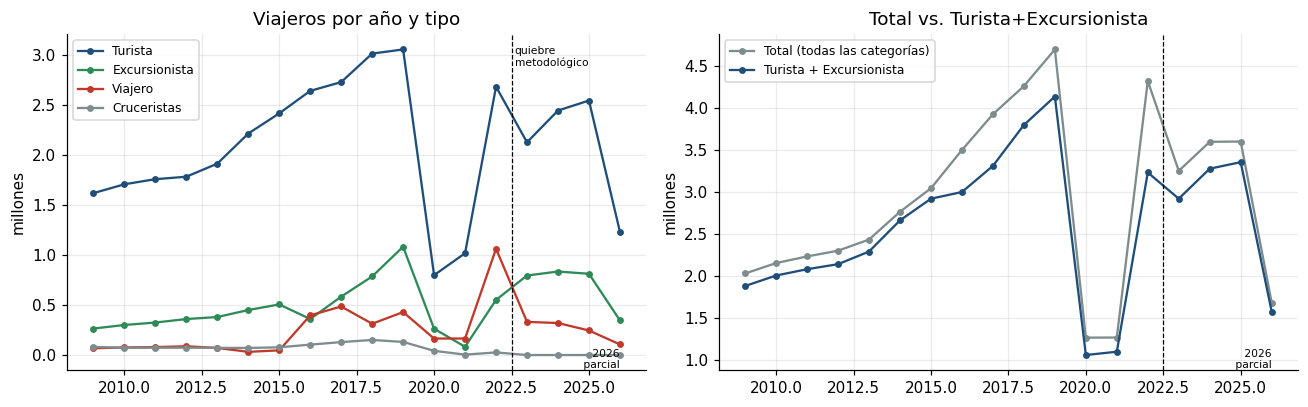
\includegraphics[width=\textwidth]{fig/eda_tipos_anual.png}
\caption{Viajeros por año y tipo (izquierda) y comparación entre el total crudo y
Turista + Excursionista (derecha). La línea punteada marca el quiebre metodológico de 2023.
El total agregado aparenta caer un 25\% entre 2022 y 2023, cuando Turista + Excursionista
solo se mueve de 3.23~M a 2.92~M.}
\end{figure}

\textbf{Decisión metodológica.} La \textbf{serie obligatoria} se construye como
\textbf{Turista + Excursionista}, las dos únicas categorías consistentes en los 210 meses.
Modelar el total crudo produciría un modelo que confunde un cambio de definición administrativa
con una caída de demanda turística, y todo pronóstico heredaría ese sesgo.

%======================= 2. EDA =======================
\seccion{Análisis exploratorio (punto 1)}

\subseccion{Calidad de los datos: faltantes, duplicados y atípicos}

\textbf{Valores faltantes.} No existe ningún valor nulo ni cadena vacía en las 13 columnas. Sin
embargo, la ausencia de \texttt{NaN} no implica ausencia de faltantes: hay faltantes
\textit{codificados como texto} (\texttt{'0'}, \texttt{'0x2a'}) en las variables geográficas,
un patrón típico de exportación de sistema. Afectan al \textbf{0.05\% del volumen}, por lo que
no alteran ninguna conclusión.

\textbf{Duplicados.} No hay duplicados exactos. Las 22 filas que se repiten según la llave
lógica (año, mes, vía, frontera, país, tipo) \textbf{no son duplicados reales}: difieren en
\textit{Agrupación Residencia}, una columna etiquetada de forma inconsistente en el tramo
2020--2022 (España aparece a la vez como \textit{España}, \textit{Otros Europa} y
\textit{Resto de mundo}). Eliminarlas restaría viajeros que sí existen. \textbf{No se eliminan}:
como todas las series se construyen agregando por suma, esas filas se consolidan solas y el
total se conserva exacto. Sí se descarta \textit{Agrupación Residencia} como variable de
análisis por poco confiable.

\textbf{Valores atípicos.} Un atípico en una serie de tiempo no es un valor extremo del
histograma, sino uno que se aparta de lo que la propia serie predice dadas su tendencia y su
estacionalidad. Por eso se compararon dos criterios, y la diferencia entre ambos es
instructiva:

\begin{itemize}[leftmargin=1.4em,itemsep=2pt]
  \item El \textbf{rango intercuartílico sobre el valor crudo} detecta \textbf{un solo punto}
  (diciembre 2019, el máximo histórico) y \textbf{no detecta ningún mes de la pandemia}. La
  serie tiene tendencia y estacionalidad tan fuertes que su rango intercuartílico es enorme:
  los \textasciitilde10 mil viajeros de abril 2020 caen dentro de ese rango amplísimo aunque
  sean absurdos para un mes de abril.
  \item El criterio basado en \textbf{residuos de una descomposición STL} ---que descuenta
  primero tendencia y estacionalidad--- identifica correctamente \textbf{siete meses
  consecutivos, de abril a octubre de 2020}, con abril 2020 a 7 desviaciones estándar de lo
  esperado.
\end{itemize}

\textbf{Conclusión práctica:} estos atípicos \textbf{no son errores y no deben eliminarse ni
imputarse}. Son un choque exógeno real y agrupado en el tiempo. Eliminarlos sería borrar el
evento más informativo de la serie.

\begin{figure}[H]
\centering
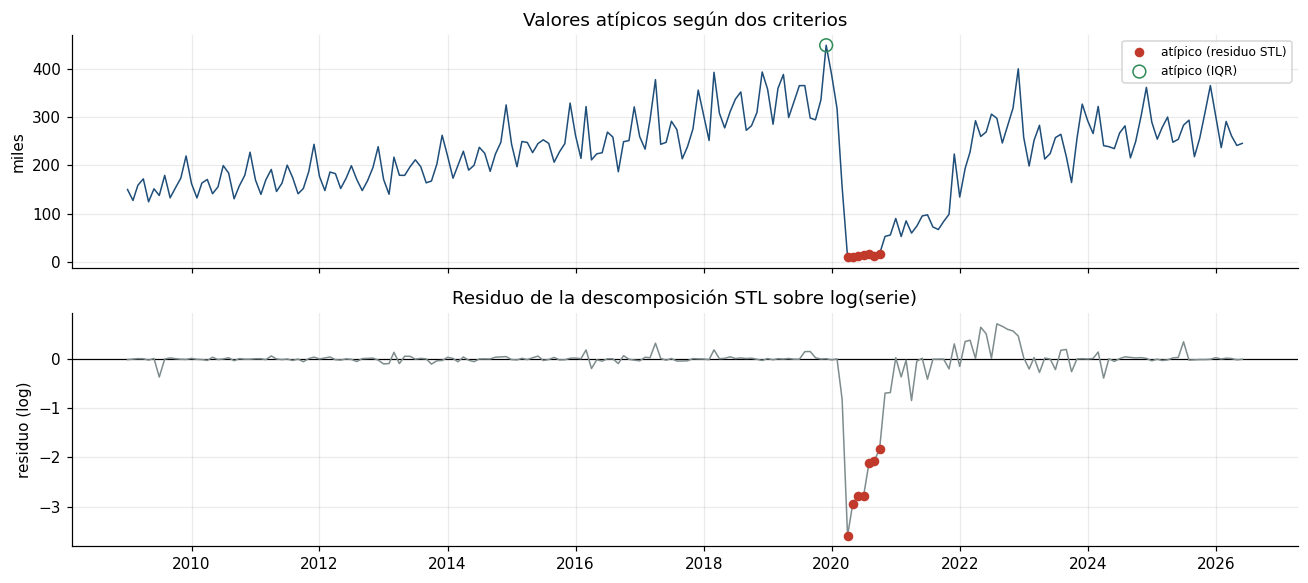
\includegraphics[width=0.96\textwidth]{fig/eda_outliers.png}
\caption{Valores atípicos según los dos criterios. El IQR sobre el valor crudo (círculos
verdes) no detecta la pandemia; el residuo STL (puntos rojos) sí.}
\end{figure}

\subseccion{Comportamiento temporal}

\begin{figure}[H]
\centering
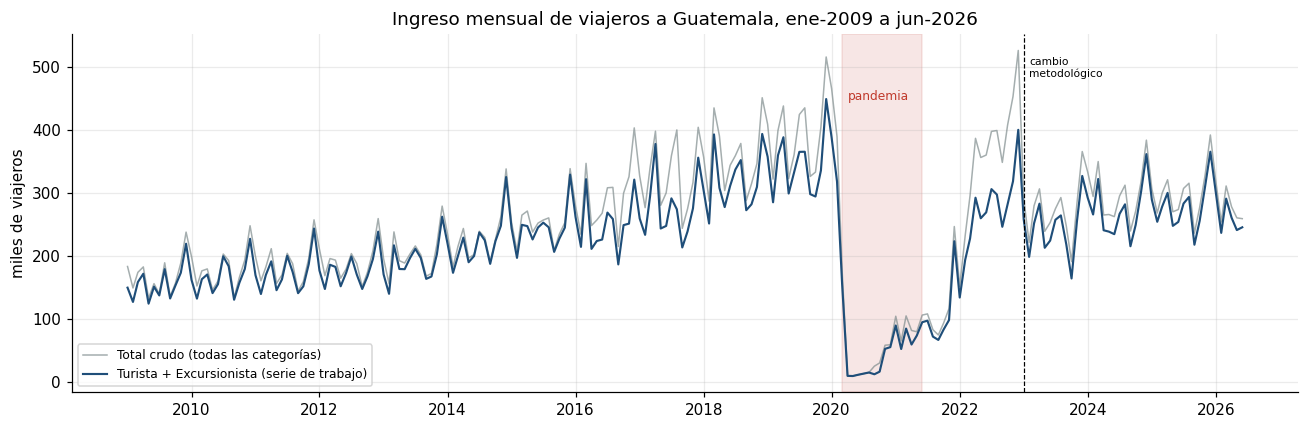
\includegraphics[width=\textwidth]{fig/eda_serie_total.png}
\caption{Ingreso mensual de viajeros, enero 2009 -- junio 2026.}
\end{figure}

A primera vista la serie muestra cuatro rasgos:

\begin{enumerate}[leftmargin=1.5em,itemsep=2pt]
  \item \textbf{Tendencia creciente y sostenida 2009--2019}, de \textasciitilde1.88~M a
  \textasciitilde4.13~M de visitantes anuales ($+120\%$ en once años, \textbf{8.19\% anual
  compuesto}).
  \item \textbf{Estacionalidad marcada y estable}, con picos que se repiten cada 12 meses.
  \item \textbf{Un choque abrupto en marzo--abril 2020}: no es un atípico aislado sino un
  cambio de nivel que dura unos 15 meses.
  \item \textbf{Recuperación en forma de escalón} desde mediados de 2021, que se estabiliza en
  un nivel \textbf{inferior} al de 2019.
\end{enumerate}

Además, la amplitud de las oscilaciones \textbf{crece con el nivel} de la serie: primer indicio
de varianza no constante, que se formaliza en la sección \ref{sec:varianza}.

\subseccion{Impacto y recuperación de la pandemia}

\begin{figure}[H]
\centering
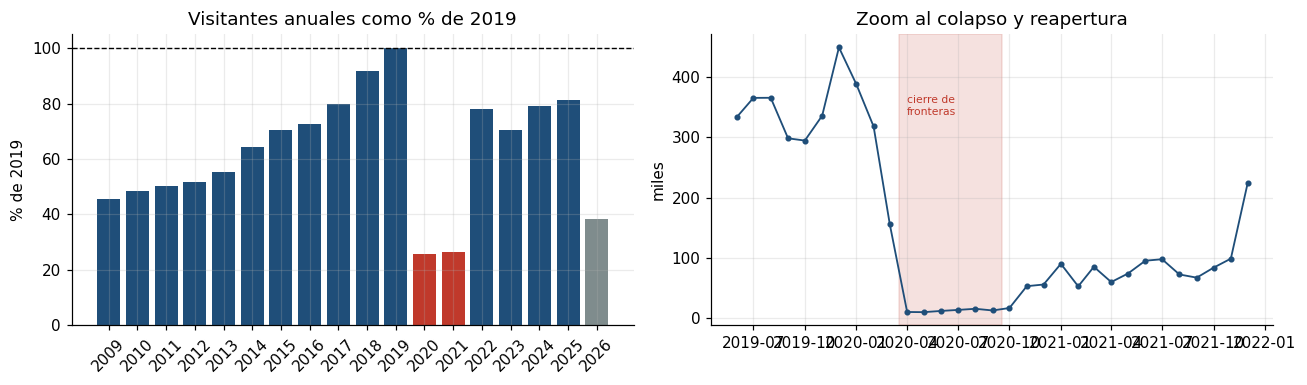
\includegraphics[width=\textwidth]{fig/eda_recuperacion.png}
\caption{Visitantes anuales como porcentaje del nivel de 2019 (izquierda) y detalle del
colapso y la reapertura (derecha).}
\end{figure}

Abril y mayo de 2020 son el fondo absoluto: \textbf{97\% menos} visitantes que el mismo mes del
año anterior (\textasciitilde10 mil frente a \textasciitilde389 mil). 2020 y 2021 cierran ambos
en torno al \textbf{26\% del nivel de 2019}.

Un hallazgo que solo aparece al desagregar: \textbf{entre abril y agosto de 2020 el 100\% de los
ingresos registrados corresponde a residentes de Guatemala}. El ingreso de extranjeros fue
exactamente cero durante el cierre de fronteras. Ese piso de 10--15 mil mensuales no es turismo
residual: es repatriación.

Medida sobre la serie tal como viene en la base, la recuperación parece \textbf{incompleta}:
2022 llega al 78\% y 2025 ---seis años después--- se queda en el \textbf{81\%} del nivel de
2019. \textbf{Pero esa cifra es engañosa}, y conviene desactivarla de inmediato porque es el
error de lectura más fácil de cometer con estos datos.

El 2019 de esa comparación \textbf{sí} contabiliza a los residentes de Guatemala que retornan;
el 2025 \textbf{no}, porque la metodología dejó de contarlos en 2023. Se está comparando una
definición ancha contra una estrecha. En 2019 esos residentes eran \textbf{1{,}703{,}434
personas, el 41\% del total}. Si se los excluye también de 2019, de modo que ambos años queden
bajo la misma definición, el resultado se invierte:

\begin{table}[H]
\centering
\small
\begin{tabular}{lrrr}
\toprule
\textbf{Base de comparación} & \textbf{2019} & \textbf{2025} & \textbf{2025 / 2019} \\
\midrule
Cruda (definiciones distintas) & 4{,}128{,}896 & 3{,}351{,}497 & 81.2\% \\
Homogénea (sin residentes de Guatemala en ambos años) & 2{,}425{,}462 & 3{,}351{,}497 & \textbf{138.2\%} \\
\bottomrule
\end{tabular}
\caption{La ``caída del 19\%'' del turismo es un artefacto del cambio de definición. A
definición constante, 2025 supera a 2019 en un 38\%.}
\end{table}

\textbf{El turismo extranjero sí se recuperó y superó el nivel prepandemia}: +38\% sobre 2019,
equivalente a un 5.5\% anual compuesto en seis años, coherente con el 8.19\% de la etapa
2009--2019 descontando los dos años perdidos. Lo que no se recuperó ---porque dejó de medirse---
es el flujo de guatemaltecos retornantes.

Esto no invalida el modelado, pero sí precisa su interpretación: la serie que se modela
\textbf{sí tiene un cambio de nivel permanente} y el modelo debe absorberlo, solo que su causa
es \textbf{administrativa y no de demanda}. Un modelo que extrapole la tendencia 2009--2019
sobrestimará la serie, pero no porque el turismo se haya estancado, sino porque a partir de 2023
la serie mide una población más pequeña.

\subseccion{Países, regiones, vías y fronteras}

Todos los rankings se calculan sobre el \textbf{total acumulado del período completo}, como pide
el enunciado.

\begin{figure}[H]
\centering
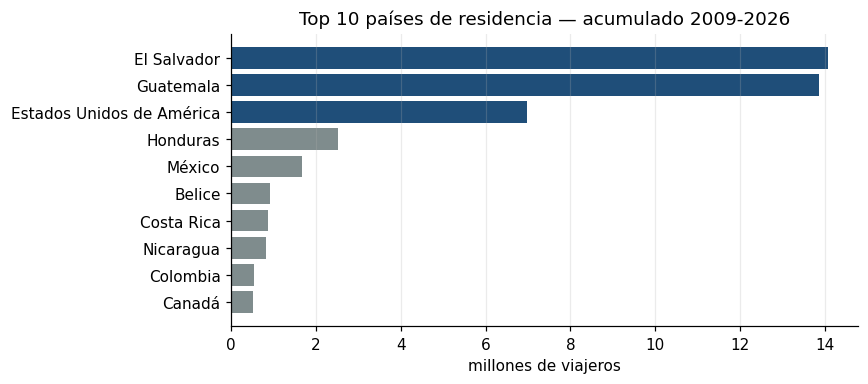
\includegraphics[width=0.78\textwidth]{fig/eda_paises.png}
\caption{Top 10 países de residencia, acumulado 2009--2026.}
\end{figure}

\textbf{Países.} El Salvador (14.1~M, 30.1\%), Guatemala (13.9~M, 29.7\%) y Estados Unidos
(7.0~M, 14.9\%) concentran el \textbf{74.7\%} del flujo; más de 200 países aportan el 25\%
restante. El perfil del crecimiento es \textbf{regional y terrestre}, no de larga distancia:
El Salvador y Honduras ganan peso mientras la cuota de Estados Unidos se contrae.

\begin{figure}[H]
\centering
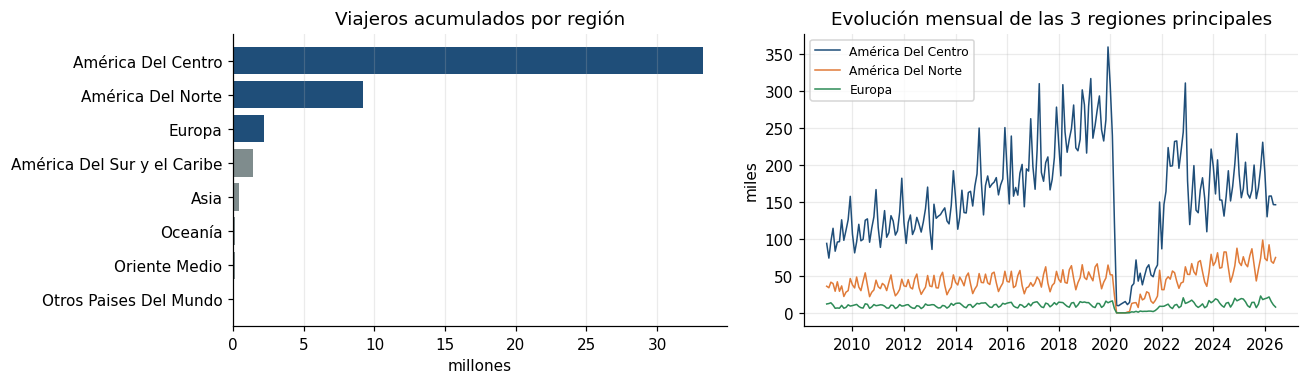
\includegraphics[width=\textwidth]{fig/eda_regiones.png}
\caption{Viajeros acumulados por región y evolución mensual de las tres principales.}
\end{figure}

\textbf{Regiones.} América Central (33.3~M, 71.3\%), América del Norte (9.2~M, 19.6\%) y
Europa (2.1~M, 4.6\%) explican el \textbf{95.5\%} del flujo. Los tres perfiles son muy distintos
---vía predominante, amplitud estacional y velocidad de recuperación--- y por eso conviene
modelarlos por separado en lugar de confiar solo en el agregado.

\begin{figure}[H]
\centering
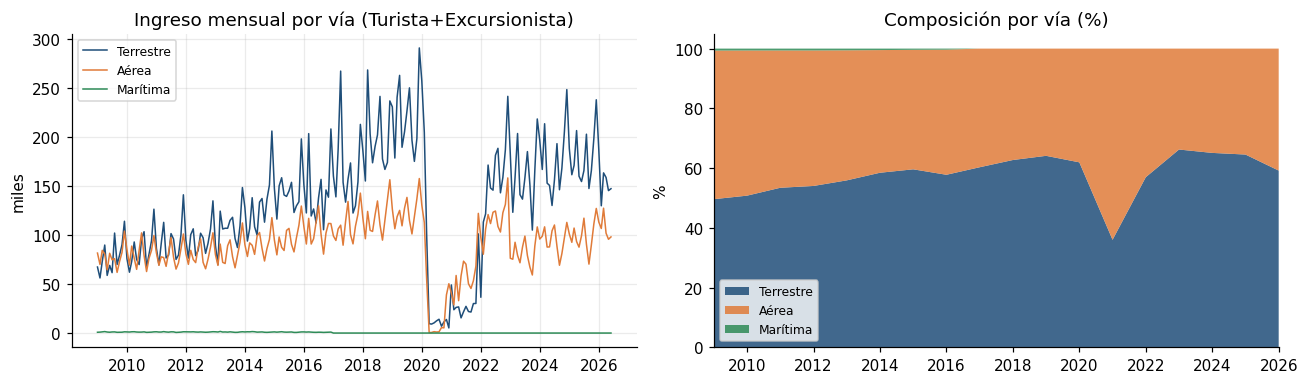
\includegraphics[width=\textwidth]{fig/eda_vias.png}
\caption{Ingreso mensual por vía y composición porcentual por año.}
\end{figure}

\textbf{Vías.} Medido sobre visitantes, la vía \textbf{terrestre domina con 59.1\%}, seguida de
la \textbf{aérea (40.7\%)} y una \textbf{marítima residual (0.2\%)}. La composición no es
estática: la terrestre gana peso hasta 2019, salvo en 2021, cuando la aérea la supera (703 mil
frente a 395 mil) porque los cierres fronterizos terrestres duraron más que la reapertura del
aeropuerto. Buen ejemplo de que la pandemia \textbf{no afectó a todas las series por igual}.

\begin{figure}[H]
\centering
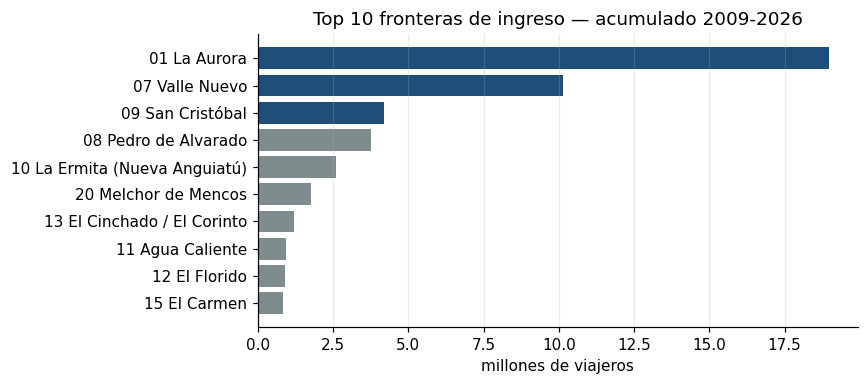
\includegraphics[width=0.78\textwidth]{fig/eda_fronteras.png}
\caption{Top 10 fronteras de ingreso, acumulado 2009--2026.}
\end{figure}

\textbf{Fronteras.} El flujo está muy concentrado: La Aurora (19.0~M, 40.7\%), Valle Nuevo
(10.1~M, 21.7\%) y San Cristóbal (4.2~M, 9.0\%) absorben el \textbf{71.3\%}; las seis primeras
llegan al 88.7\%. El cruce frontera $\times$ vía confirma la lectura estructural: La Aurora
\textbf{es} el flujo aéreo (100\% de su volumen), y las cinco siguientes son terrestres, todas
sobre la línea con El Salvador y Honduras.

\subseccion{Estacionalidad y estadísticas descriptivas}

El patrón intra-anual se analiza sobre el período \textbf{pre-pandemia (2009--2019)} para que el
colapso de 2020--2021 no distorsione el perfil.

\begin{figure}[H]
\centering
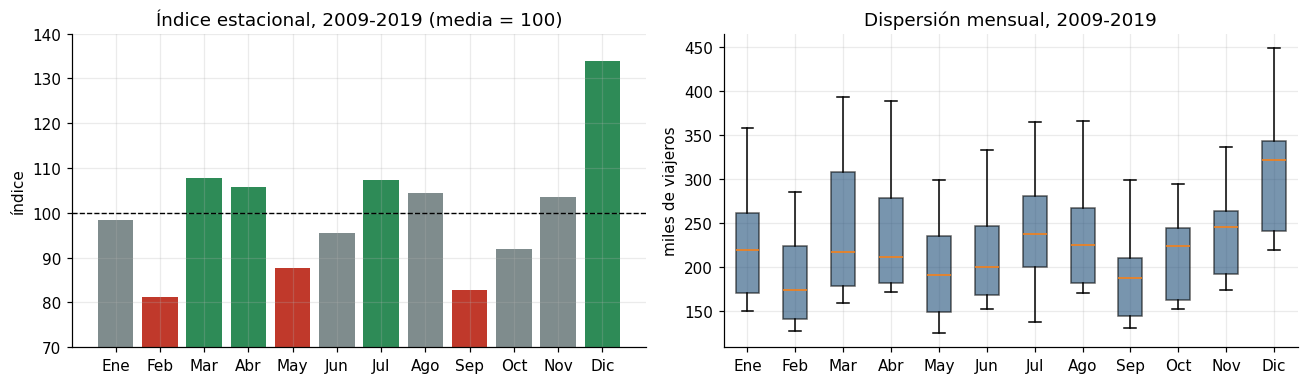
\includegraphics[width=\textwidth]{fig/eda_estacionalidad.png}
\caption{Índice estacional (promedio del año = 100) y dispersión mensual, 2009--2019.}
\end{figure}

\begin{figure}[H]
\centering
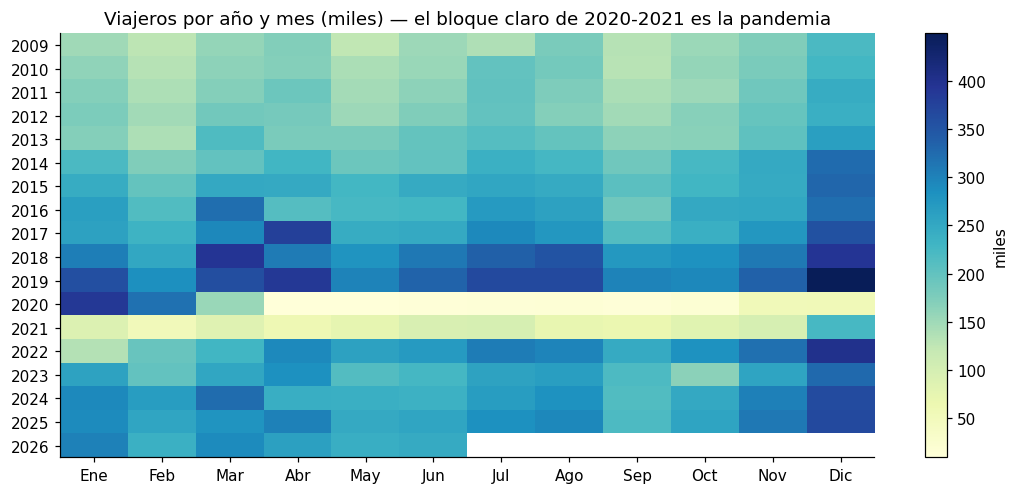
\includegraphics[width=0.88\textwidth]{fig/eda_heatmap.png}
\caption{Viajeros por año y mes. El bloque claro de 2020--2021 es la pandemia.}
\end{figure}

El patrón es nítido y \textbf{muy estable año con año}:

\begin{itemize}[leftmargin=1.4em,itemsep=2pt]
  \item \textbf{Diciembre es el máximo absoluto (índice 134)}: fiestas de fin de año y visita
  de la diáspora.
  \item \textbf{Marzo--abril (108 / 106)}: Semana Santa. Al ser una \textbf{fiesta móvil}, en
  algunos años el pico cae en marzo y en otros en abril, lo que introduce ruido que un modelo
  estacional de período fijo (12) no captura del todo.
  \item \textbf{Julio--agosto (107 / 104)}: vacaciones de mitad de año.
  \item \textbf{Los mínimos son febrero (81) y septiembre (83)}, ambos \textasciitilde20\% por
  debajo del promedio.
\end{itemize}

La amplitud entre el mejor y el peor mes es de \textbf{52.6 puntos}: la componente estacional es
económicamente relevante, no un detalle estadístico. El mapa de calor muestra además que el
patrón \textbf{sobrevive intacto a la pandemia; el nivel no}.

%======================= 3. SERIES Y PARTICION =======================
\seccion{Construcción de las series y partición (puntos 2 y 3)}

\subseccion{Criterio de selección de las categorías}

El enunciado pide elegir \textbf{dos} categorías de análisis. El criterio aplicado fue el único
defendible a la luz del exploratorio: \textbf{sirve la categoría cuyas series existan y sean
comparables en los 210 meses}.

\begin{table}[H]
\centering
\small
\begin{tabularx}{\textwidth}{lcX}
\toprule
\textbf{Categoría} & \textbf{¿Utilizable?} & \textbf{Razón} \\
\midrule
Fronteras & \textbf{Sí} & Definidas físicamente; las tres principales tienen serie completa. \\
Regiones (\textit{Región dos}) & \textbf{Sí} & Completas; absorben el quiebre de 2023 de forma explicable. \\
Países de residencia & Con reservas & Cambio de granularidad en 2023; \texttt{Guatemala} termina en 2022. \\
Vías de ingreso & \textbf{No} & Marítima en cero desde 2017 y cruceros fuera de la base desde 2023: dos quiebres encadenados. \\
Tipo de viajero & \textbf{No} & \texttt{Cruceristas} desaparece en 2023 y \texttt{Viajero} sufre el quiebre de definición. \\
\bottomrule
\end{tabularx}
\caption{Evaluación de las cinco categorías propuestas por el enunciado.}
\end{table}

\textbf{Selección:} \textbf{Fronteras} (Top 3 acumulado) y \textbf{Regiones geográficas}
(Top 3 de \textit{Región dos}). Además de ser las más limpias, son las dos más útiles para el
INGUAT: una responde a \textit{por dónde entra} la gente (capacidad operativa) y la otra a
\textit{de dónde viene} (promoción de mercados).

\subseccion{Las siete series}

\begin{table}[H]
\centering
\small
\begin{tabular}{lrrrrr}
\toprule
\textbf{Serie} & \textbf{Inicio} & \textbf{Fin} & \textbf{Frec.} & \textbf{n} & \textbf{Meses en 0} \\
\midrule
Total (Turista + Excursionista) & 2009-01 & 2026-06 & Mensual & 210 & 0 \\
Frontera: La Aurora             & 2009-01 & 2026-06 & Mensual & 210 & 0 \\
Frontera: Valle Nuevo           & 2009-01 & 2026-06 & Mensual & 210 & 0 \\
Frontera: San Cristóbal         & 2009-01 & 2026-06 & Mensual & 210 & 0 \\
Región: América Del Centro      & 2009-01 & 2026-06 & Mensual & 210 & 0 \\
Región: América Del Norte       & 2009-01 & 2026-06 & Mensual & 210 & 5 \\
Región: Europa                  & 2009-01 & 2026-06 & Mensual & 210 & 5 \\
\bottomrule
\end{tabular}
\caption{Inciso 4.a: inicio, fin y frecuencia de cada serie. Las tres fronteras del Top~3 son
La Aurora, Valle Nuevo y San Cristóbal; las tres regiones son América del Centro, América del
Norte y Europa, todas por total acumulado del período completo. Los 5 meses en cero de América
del Norte y Europa son abril--agosto de 2020: ceros reales por cierre de fronteras, no datos
faltantes.}
\end{table}

\begin{table}[H]
\centering
\small
\begin{tabular}{lrrrrr}
\toprule
\textbf{Serie} & \textbf{Media} & \textbf{Desv. est.} & \textbf{CV \%} & \textbf{Mín} & \textbf{Máx} \\
\midrule
Total (Turista + Excursionista) & 222{,}341 & 84{,}673 & 38.1 & 9{,}779 & 448{,}790 \\
Frontera: La Aurora             & 90{,}418  & 27{,}774 & 30.7 & 484 & 158{,}073 \\
Frontera: Valle Nuevo           & 48{,}292  & 23{,}448 & 48.6 & 80 & 111{,}127 \\
Frontera: San Cristóbal         & 19{,}916  & 11{,}392 & 57.2 & 14 & 53{,}120 \\
Región: América Del Centro      & 158{,}467 & 66{,}473 & 41.9 & 9{,}779 & 359{,}152 \\
Región: América Del Norte       & 43{,}605  & 17{,}880 & 41.0 & 0 & 98{,}361 \\
Región: Europa                  & 10{,}210  & 4{,}391  & 43.0 & 0 & 22{,}799 \\
\bottomrule
\end{tabular}
\caption{Estadísticas descriptivas de las siete series (viajeros por mes).}
\end{table}

\begin{figure}[H]
\centering
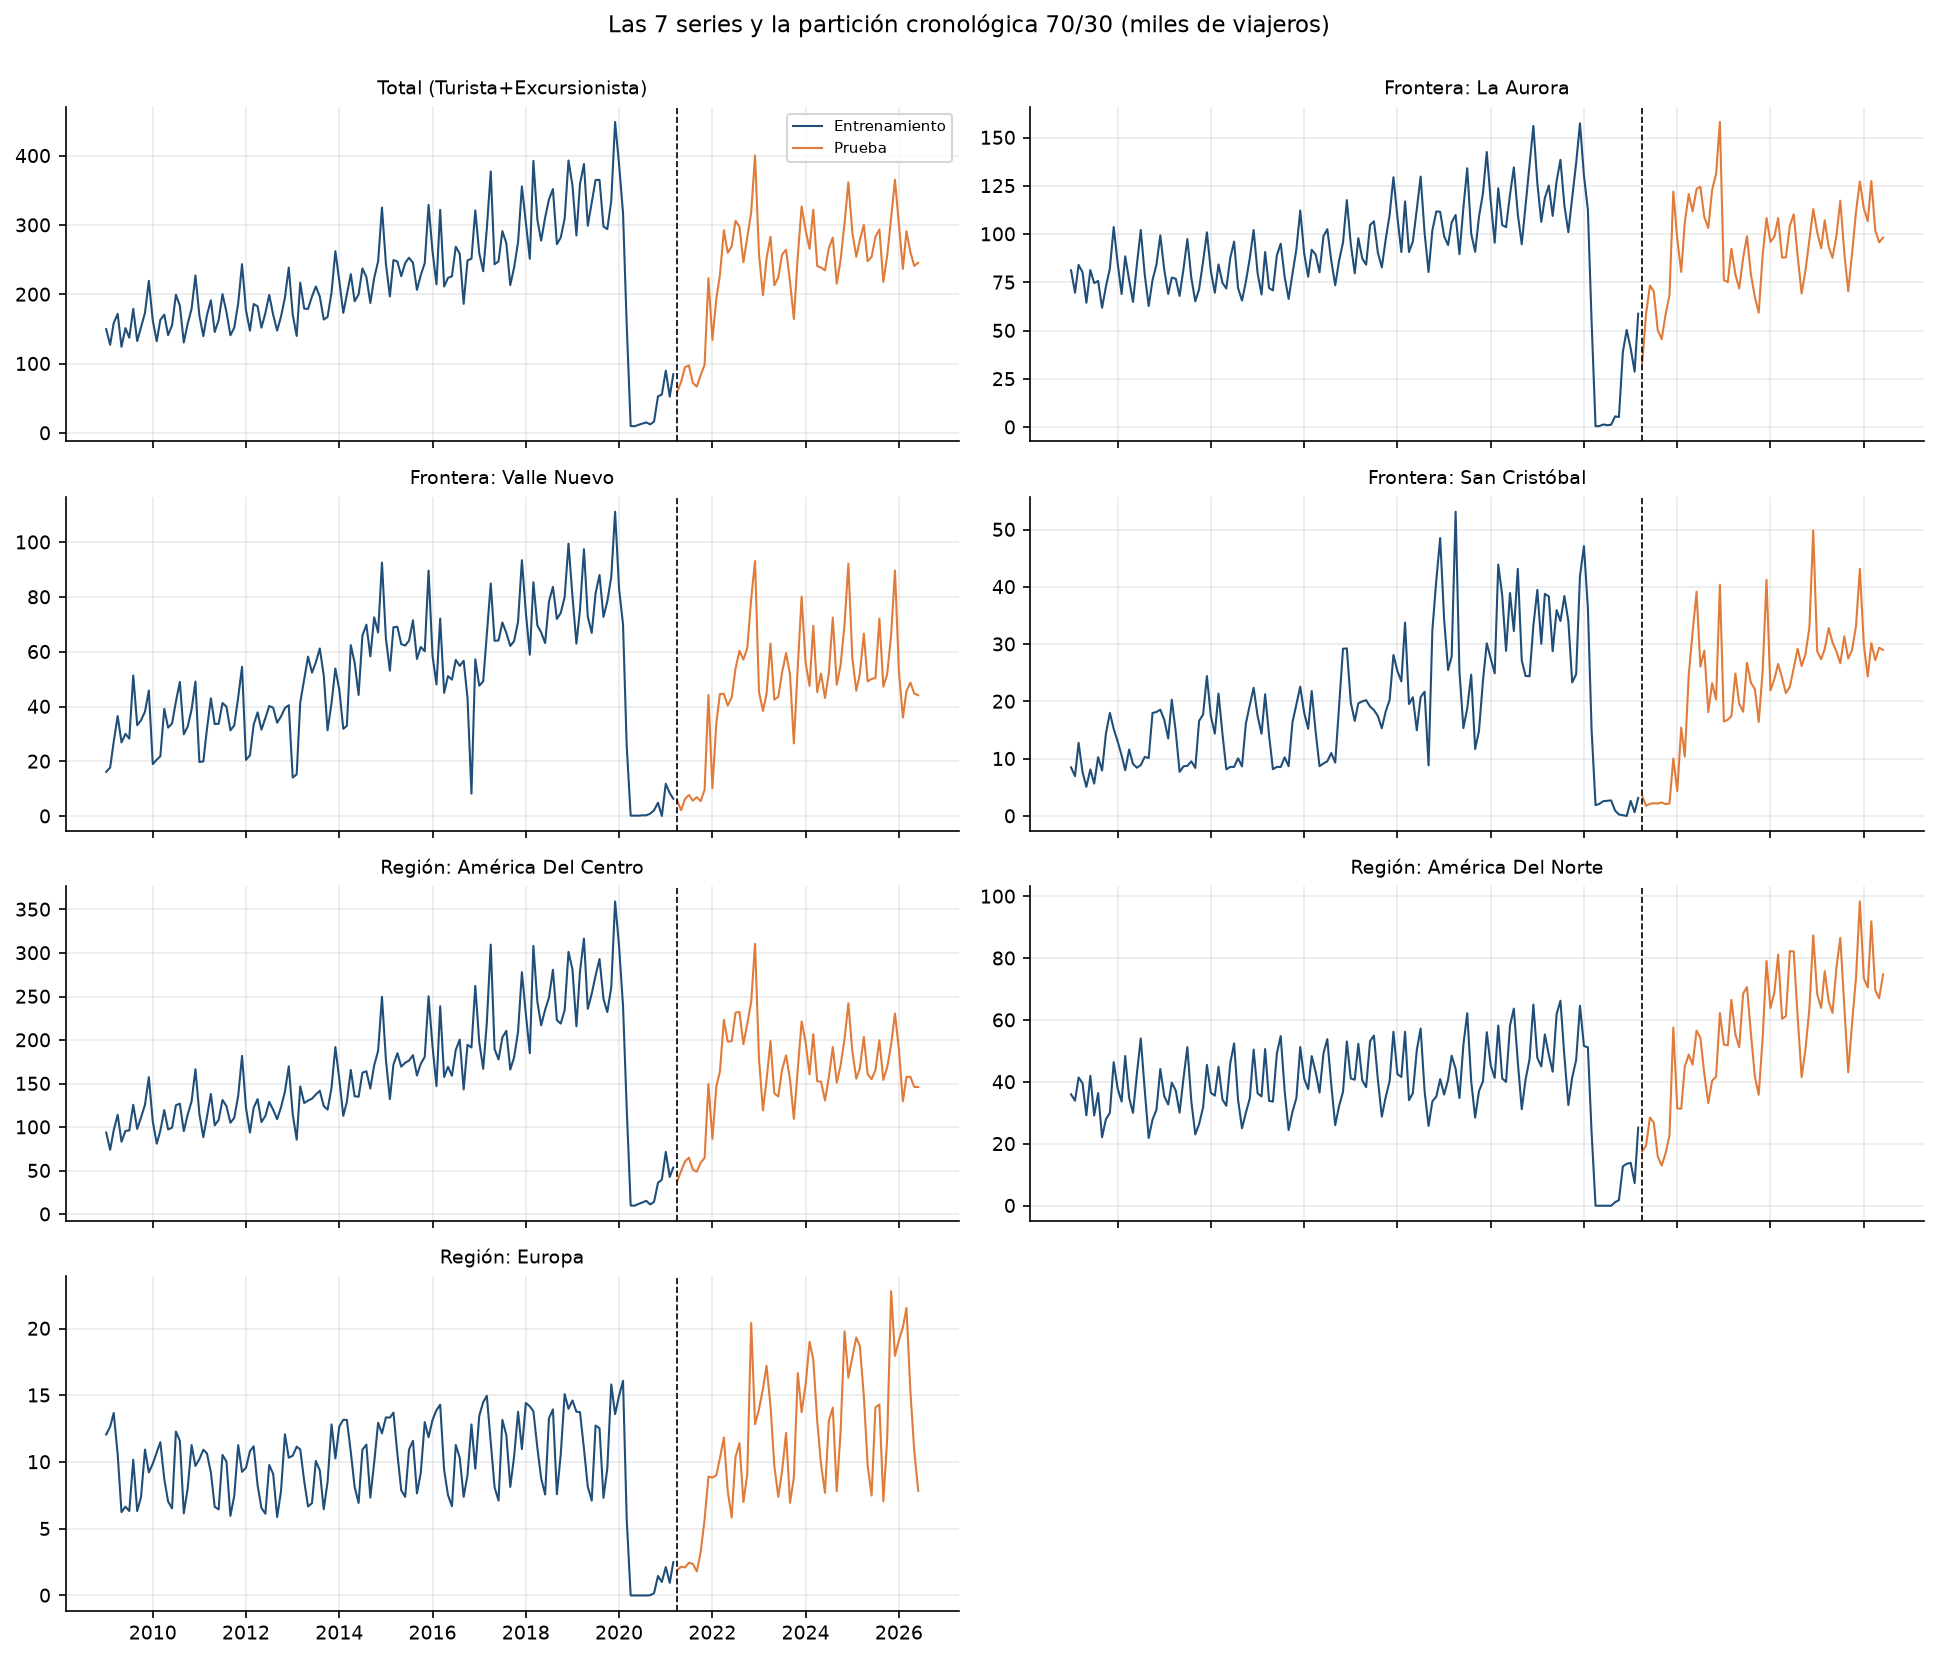
\includegraphics[width=\textwidth]{fig/20_split_todas.png}
\caption{Las siete series y la partición cronológica 70/30.}
\end{figure}

\subseccion{Partición 70 / 30}

El corte es \textbf{cronológico}, nunca aleatorio: usar datos del futuro para predecir el pasado
es fuga de información y produce métricas de error optimistas y falsas.

\begin{table}[H]
\centering
\small
\begin{tabular}{lccc}
\toprule
\textbf{Conjunto} & \textbf{Desde} & \textbf{Hasta} & \textbf{Meses} \\
\midrule
Entrenamiento (70\%) & 2009-01 & 2021-03 & 147 \\
Prueba (30\%)        & 2021-04 & 2026-06 & 63 \\
\bottomrule
\end{tabular}
\caption{Partición cronológica de las 210 observaciones.}
\end{table}

\textbf{Advertencia central del informe.} El corte al 70\% cae en \textbf{abril de 2021}, es
decir, \textbf{dentro del hueco pandémico}. El conjunto de entrenamiento termina en el piso del
colapso y el de prueba contiene toda la recuperación.

Es una partición \textbf{dura pero honesta}: ningún modelo entrenado hasta esa fecha puede
anticipar la reapertura de fronteras, porque esa información sencillamente no está en los datos
de entrenamiento. Los errores del conjunto de prueba serán altos \textbf{por construcción}, y un
MAE o RMSE elevado \textbf{no} implica que el modelo esté mal especificado. Se respeta el 70/30
que pide el enunciado y en la sección~\ref{sec:control} se reporta una partición alternativa
post-pandemia que separa el error atribuible al choque exógeno del error propio del modelo.

%======================= 4. ANALISIS DE LAS SERIES =======================
\seccion{Análisis de las series (punto 4)}

Todas las series recibieron idéntico tratamiento, de modo que los resultados sean comparables
entre sí. Esta sección resume los hallazgos transversales y luego detalla cada serie.

\subseccion{Descomposición, tendencia y estacionalidad}

Se descompuso cada serie con \textbf{STL} sobre $\log(1+x)$ y se midió la fuerza de cada
componente con los índices de Wang, Smith y Hyndman:
\[
F_T = \max\!\left(0,\; 1 - \frac{\mathrm{Var}(R_t)}{\mathrm{Var}(T_t + R_t)}\right),
\qquad
F_S = \max\!\left(0,\; 1 - \frac{\mathrm{Var}(R_t)}{\mathrm{Var}(S_t + R_t)}\right).
\]

\textbf{Una precisión metodológica importante.} Calculados sobre la muestra completa, estos
índices resultan engañosamente bajos: para la serie total dan $F_T=0.35$ y $F_S=0.05$, cifras
que sugerirían una serie casi sin tendencia ni estacionalidad, en contradicción directa con lo
que muestra el gráfico. La causa es que \textbf{el residuo de la pandemia domina la varianza
total} y hunde ambos cocientes. Medidos sobre la ventana limpia \textbf{2009--2019}, los mismos
índices dan $F_T=0.94$ y $F_S=0.80$, que sí describen la serie. Por eso \textbf{todas las
medidas de caracterización de este informe se calculan sobre 2009--2019}, y el impacto de la
pandemia se mide aparte con estadísticos propios.

\begin{table}[H]
\centering
\small
\begin{tabular}{lcccc}
\toprule
& \multicolumn{2}{c}{\textbf{2009--2019 (limpio)}} & \multicolumn{2}{c}{\textbf{2009--2026 (con pandemia)}} \\
\cmidrule(lr){2-3}\cmidrule(lr){4-5}
\textbf{Serie} & $F_T$ & $F_S$ & $F_T$ & $F_S$ \\
\midrule
Total (Turista + Excursionista) & 0.941 & 0.795 & 0.348 & 0.047 \\
Frontera: La Aurora             & 0.926 & 0.874 & 0.145 & 0.049 \\
Frontera: Valle Nuevo           & 0.672 & 0.421 & 0.485 & 0.059 \\
Frontera: San Cristóbal         & 0.833 & 0.706 & 0.650 & 0.129 \\
Región: América Del Centro      & 0.950 & 0.805 & 0.550 & 0.077 \\
Región: América Del Norte       & 0.701 & 0.882 & 0.119 & 0.009 \\
Región: Europa                  & 0.600 & 0.880 & 0.281 & 0.076 \\
\bottomrule
\end{tabular}
\caption{Fuerza de tendencia y estacionalidad. La caída al incluir 2020--2021 no significa que
las series pierdan tendencia o estacionalidad: es un artefacto de la varianza del choque.}
\end{table}

\textbf{Lectura.} Las siete series tienen \textbf{tendencia fuerte} ($F_T \geq 0.60$) y
\textbf{estacionalidad relevante} ($F_S \geq 0.42$). Que una serie tenga estacionalidad
significa que el mes del año es un predictor por sí mismo, y por tanto que un modelo sin
términos estacionales está condenado a errar de forma sistemática y repetitiva. Que tenga
tendencia significa que la media no es constante, y por tanto que la serie no puede ser
estacionaria en media sin diferenciar.

\subseccion{Estacionariedad en varianza y transformación}
\label{sec:varianza}

Se evaluó con tres diagnósticos complementarios sobre 2009--2019: la correlación entre la media
móvil y la desviación estándar móvil de 12 meses, la pendiente de $\log(\mathrm{sd})$ contra
$\log(\mathrm{media})$ (0 indica varianza constante, 1 que la dispersión es proporcional al
nivel) y el $\lambda$ de Box-Cox.

\begin{table}[H]
\centering
\small
\begin{tabular}{lccccl}
\toprule
\textbf{Serie} & \textbf{corr(media, sd)} & \textbf{pendiente} & $\boldsymbol{\lambda}$ & \textbf{¿Transformar?} \\
\midrule
Total (Turista + Excursionista) & 0.845 & 0.871 & $-0.339$ & Sí \\
Frontera: La Aurora             & 0.873 & 0.824 & $-0.515$ & Sí \\
Frontera: Valle Nuevo           & 0.174 & 0.194 & 0.703 & No \\
Frontera: San Cristóbal         & 0.626 & 0.687 & 0.063 & Sí \\
Región: América Del Centro      & 0.810 & 0.822 & $-0.225$ & Sí \\
Región: América Del Norte       & 0.762 & 0.685 & 0.181 & Sí \\
Región: Europa                  & 0.862 & 1.164 & 0.733 & Sí \\
\bottomrule
\end{tabular}
\caption{Diagnóstico de estacionariedad en varianza (2009--2019).}
\end{table}

\textbf{Conclusión.} En seis de las siete series la dispersión crece casi proporcionalmente al
nivel (pendientes de 0.69 a 1.16) y el $\lambda$ de Box-Cox se sitúa cerca de 0, que es
exactamente el caso logarítmico. \textbf{Estas series no son estacionarias en varianza y
requieren transformación.} La única excepción es Valle Nuevo, cuya dispersión es prácticamente
independiente del nivel.

\textbf{Se modelaron todas en $\log(1+x)$}, incluida Valle Nuevo, por tres razones: estabiliza
la varianza donde hace falta, garantiza que las predicciones devueltas a la escala original sean
no negativas, y mantiene todas las series en una escala común para que la comparación sea
legítima. El $+1$ evita el $\log(0)$ de los meses de cierre total de fronteras de 2020.

\begin{figure}[H]
\centering
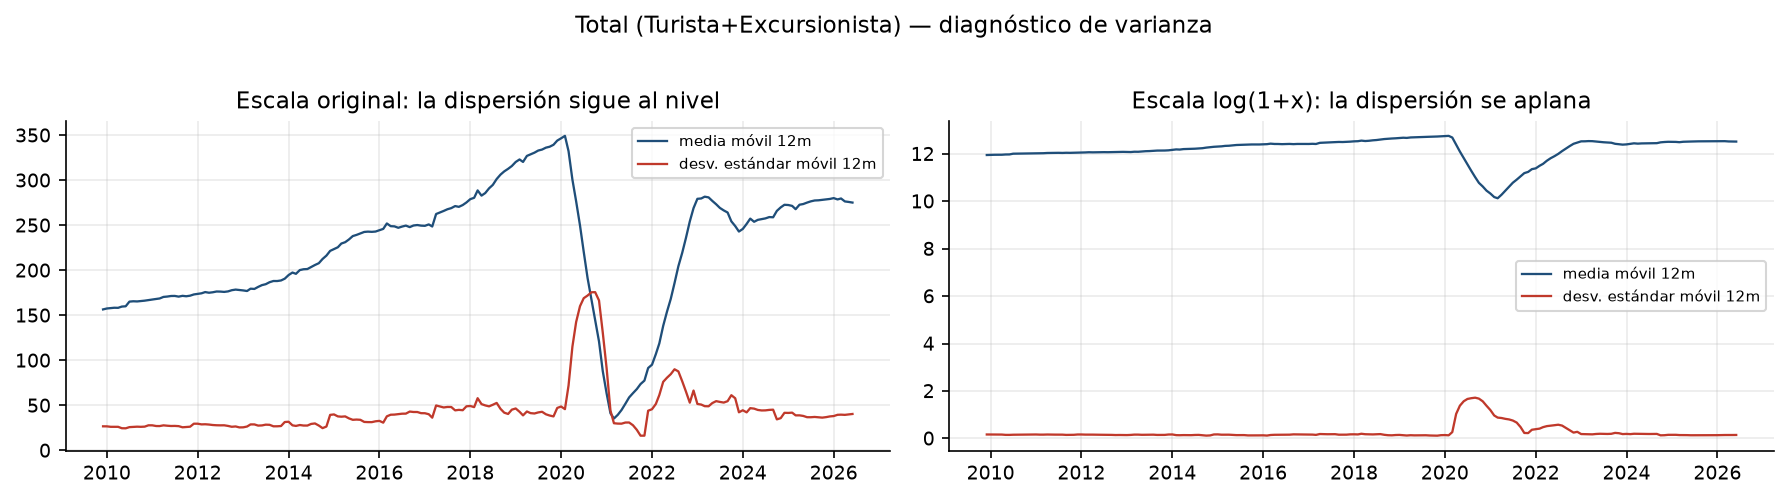
\includegraphics[width=\textwidth]{fig/22_total_varianza.png}
\caption{Serie total: en escala original la desviación móvil sigue al nivel (izquierda);
en escala logarítmica se aplana (derecha).}
\end{figure}

\subseccion{Estacionariedad en media: autocorrelación y Dickey-Fuller}

\textbf{Evidencia gráfica.} La función de autocorrelación de las series sin diferenciar
\textbf{decae muy lentamente} y se mantiene positiva y significativa durante decenas de rezagos.
Ese decaimiento lento es la firma gráfica de la \textbf{no estacionariedad en media}: si la
serie fuera estacionaria, la ACF caería rápidamente hacia cero tras unos pocos rezagos. Se
observa además un repunte en los rezagos múltiplos de 12, que corresponde a la componente
estacional anual.

\begin{figure}[H]
\centering
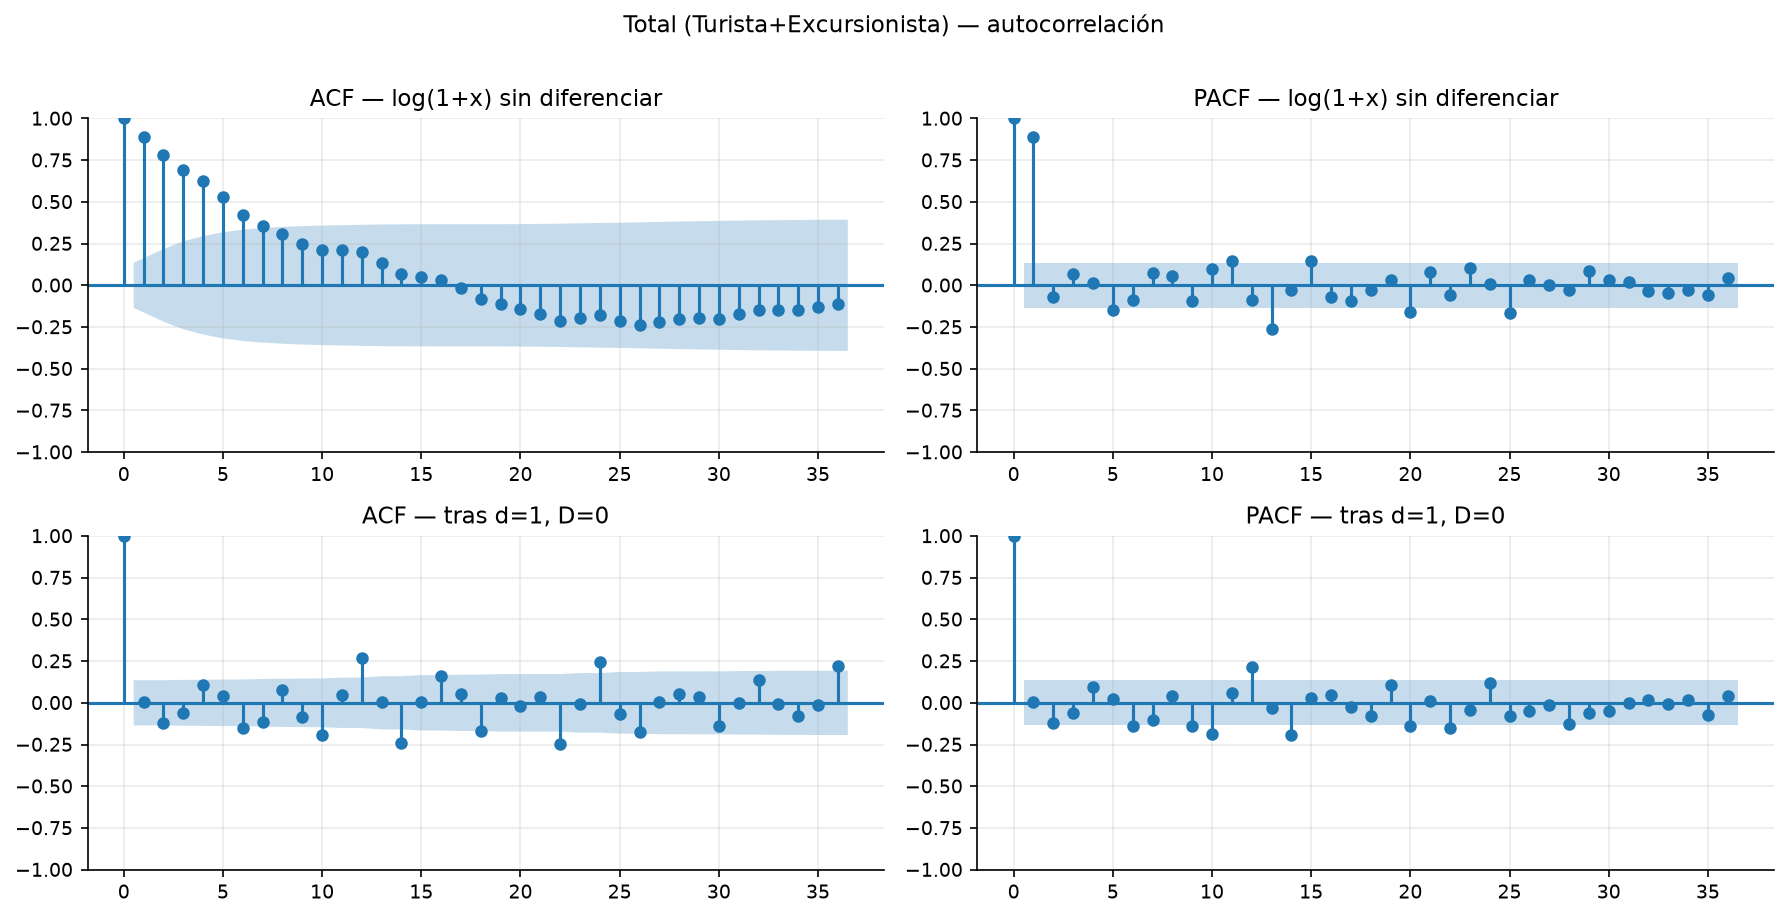
\includegraphics[width=\textwidth]{fig/23_total_acf.png}
\caption{Serie total: ACF y PACF antes (arriba) y después (abajo) de diferenciar. Arriba, el
decaimiento lento de la ACF evidencia la no estacionariedad en media; abajo, tras una
diferencia regular, la ACF cae abruptamente.}
\end{figure}

\textbf{Evidencia estadística.} Se aplicaron dos pruebas con hipótesis nulas opuestas, que es la
forma correcta de decidir: la \textbf{Dickey-Fuller aumentada} (ADF, $H_0$: hay raíz unitaria,
es decir NO estacionaria) y la \textbf{KPSS} ($H_0$: SÍ estacionaria).

\begin{table}[H]
\centering
\small
\begin{tabular}{lcccc}
\toprule
\textbf{Serie} & \textbf{ADF original} & \textbf{ADF log} & \textbf{ADF log + 1 dif.} & $\boldsymbol{d}$ \\
\midrule
Total (Turista + Excursionista) & 0.0470 & 0.0833 & 0.0001 & 1 \\
Frontera: La Aurora             & 0.0185 & 0.0077 & 0.0000 & 0 \\
Frontera: Valle Nuevo           & 0.0344 & 0.0185 & 0.0000 & 0 \\
Frontera: San Cristóbal         & 0.2330 & 0.0235 & 0.0000 & 0 \\
Región: América Del Centro      & 0.0448 & 0.0544 & 0.0002 & 1 \\
Región: América Del Norte       & 0.2196 & 0.0393 & 0.0000 & 0 \\
Región: Europa                  & 0.0222 & 0.0231 & 0.0000 & 0 \\
\bottomrule
\end{tabular}
\caption{Valores $p$ de la prueba de Dickey-Fuller aumentada y número de diferencias regulares
resultante. Un $p < 0.05$ permite rechazar la raíz unitaria.}
\end{table}

\textbf{Qué hay que hacer para volverlas estacionarias en media.} \textbf{Diferenciar}. En las
dos series agregadas (Total y América del Centro) la ADF no permite rechazar la raíz unitaria en
la escala logarítmica ($p = 0.083$ y $p = 0.054$), y una sola diferencia regular basta para que
el $p$ caiga a 0.0001 o menos: \textbf{$d = 1$}. En las cinco restantes la ADF ya rechaza la
raíz unitaria en la serie transformada, de modo que \textbf{$d = 0$} y la estacionariedad en
media se consigue solo con la transformación logarítmica.

Este resultado merece una advertencia: la forma en V de la pandemia ---caída brusca seguida de
recuperación--- hace que la serie \textit{parezca} revertir a la media y vuelve el resultado de
la ADF sensible a esa ventana. Por eso se contrastó con la \textbf{KPSS}, que no rechaza la
estacionariedad en ningún caso tras la transformación, y por eso se incluyeron de todos modos
modelos con diferenciación entre los candidatos: la decisión final se tomó comparando el ajuste
real, no un único valor $p$.

\textbf{Diferenciación estacional.} Se aplicó la prueba \textbf{OCSB} de raíz unitaria
estacional. Devuelve $D = 0$ para cinco series y $D = 1$ para América del Norte y Europa. Que
la OCSB devuelva 0 no contradice la fuerte estacionalidad detectada: la prueba busca una raíz
unitaria \textit{estacional} (una estacionalidad que cambia de forma aleatoria año con año), y
la de estas series es \textbf{determinista y muy estable}, por lo que se captura mejor con
términos estacionales AR/MA que diferenciando. Aun así, se incluyó siempre el modelo
``aerolínea'' $(0,1,1)(0,1,1)_{12}$ con diferenciación estacional forzada, para que fuera la
comparación empírica y no un supuesto previo la que decidiera.

\subseccion{Selección de $p$, $d$ y $q$}

Los órdenes se eligieron combinando dos fuentes. \textbf{Primero, la lectura de la ACF y la
PACF} sobre la serie ya estacionarizada: una PACF que se corta en el rezago $k$ y una ACF que
decae sugieren un AR($k$); el patrón inverso sugiere un MA; los picos en los rezagos 12 y 24
indican las componentes estacionales. \textbf{Segundo, \texttt{auto\_arima}}, forzándole los
valores de $d$ y $D$ obtenidos de las pruebas formales y dejándole optimizar $p$, $q$, $P$ y $Q$
por AIC.

\begin{table}[H]
\centering
\small
\begin{tabular}{lccl}
\toprule
\textbf{Serie} & $\boldsymbol{d}$ & $\boldsymbol{D}$ & \textbf{Propuesta de \texttt{auto\_arima}} \\
\midrule
Total (Turista + Excursionista) & 1 & 0 & SARIMA$(0,1,0)(2,0,0)_{12}$ \\
Frontera: La Aurora             & 0 & 0 & SARIMA$(1,0,1)(1,0,1)_{12}$ \\
Frontera: Valle Nuevo           & 0 & 0 & SARIMA$(1,0,1)(0,0,0)_{12}$ \\
Frontera: San Cristóbal         & 0 & 0 & SARIMA$(3,0,0)(2,0,0)_{12}$ \\
Región: América Del Centro      & 1 & 0 & SARIMA$(0,1,0)(2,0,0)_{12}$ \\
Región: América Del Norte       & 0 & 1 & SARIMA$(3,0,2)(0,1,0)_{12}$ \\
Región: Europa                  & 0 & 1 & SARIMA$(2,0,2)(0,1,0)_{12}$ \\
\bottomrule
\end{tabular}
\caption{Órdenes de diferenciación determinados por ADF y OCSB, y modelo propuesto por
\texttt{auto\_arima}.}
\end{table}

\textbf{¿Tienen sentido los modelos propuestos?} En general sí, y son interpretables:

\begin{itemize}[leftmargin=1.4em,itemsep=3pt]
  \item Para el \textbf{Total} y \textbf{América del Centro}, \texttt{auto\_arima} propone
  $(0,1,0)(2,0,0)_{12}$: un paseo aleatorio con deriva más dos términos autorregresivos
  estacionales. Es coherente con lo observado: el nivel del mes que viene se explica sobre todo
  por el de este mes (de ahí $p=q=0$ tras diferenciar), y lo que queda por explicar es el patrón
  anual, capturado por los rezagos 12 y 24.
  \item Para \textbf{La Aurora}, $(1,0,1)(1,0,1)_{12}$ combina memoria de corto plazo con
  memoria estacional, razonable para un aeropuerto con reservas anticipadas y temporadas bien
  definidas.
  \item Para \textbf{San Cristóbal}, $(3,0,0)(2,0,0)_{12}$ es un AR puro relativamente largo,
  consistente con una serie de frontera terrestre con inercia mensual alta.
  \item Para \textbf{América del Norte} y \textbf{Europa}, la diferenciación estacional
  ($D=1$) domina la especificación, coherente con series cuyo comportamiento está regido casi
  enteramente por la temporada.
\end{itemize}

\textbf{Advertencia sobre la comparación de AIC y BIC.} Estos criterios \textbf{solo son
comparables entre modelos ajustados sobre el mismo número efectivo de observaciones}.
Diferenciar consume datos: un modelo con $d=1, D=1$ evalúa su verosimilitud sobre 134
observaciones y uno con $d=1, D=0$ sobre 146. Comparar sus AIC directamente es un error
frecuente. Por eso, en las tablas siguientes se reporta la columna $n_{\text{ef}}$ y el mejor
modelo por AIC se selecciona \textbf{solo dentro del grupo que comparte ese valor}. MAE, RMSE y
MAPE, en cambio, se calculan siempre sobre el mismo conjunto de prueba y en la escala original,
por lo que sí son comparables entre todos los modelos.

%======================= 5. MODELOS Y PREDICCION =======================
\seccion{Modelos, predicción y comparación (puntos 4.g a 4.k)}

Para cada serie se ajustaron \textbf{seis modelos SARIMA} (el de \texttt{auto\_arima}, tres
variantes derivadas de la ACF/PACF y dos modelos con diferenciación estacional forzada) más los
\textbf{cuatro algoritmos alternativos} que pide el enunciado: \textbf{Prophet},
\textbf{Holt-Winters}, \textbf{suavizamiento exponencial simple} y \textbf{seasonal naive}. En
total, diez modelos por serie y setenta en el estudio.

\subseccion{Resultado global sobre la partición 70/30}

\begin{table}[H]
\centering
\small
\begin{tabular}{lccr}
\toprule
\textbf{Serie} & \textbf{Mejor modelo (RMSE)} & \textbf{MAPE \%} & \textbf{RMSE} \\
\midrule
Total (Turista + Excursionista) & Suav. exponencial simple & 60.6 & 173{,}699 \\
Frontera: La Aurora             & Suav. exponencial simple & 36.6 & 42{,}064 \\
Frontera: Valle Nuevo           & Suav. exponencial simple & 80.3 & 46{,}248 \\
Frontera: San Cristóbal         & Suav. exponencial simple & 81.5 & 23{,}721 \\
Región: América Del Centro      & Suav. exponencial simple & 61.4 & 120{,}333 \\
Región: América Del Norte       & Suav. exponencial simple & 53.4 & 36{,}714 \\
Región: Europa                  & Suav. exponencial simple & 71.4 & 10{,}689 \\
\bottomrule
\end{tabular}
\caption{Mejor modelo por RMSE sobre el conjunto de prueba 2021-04 a 2026-06.}
\end{table}

\textbf{Este resultado hay que leerlo con cuidado, porque es un artefacto de la partición.} El
suavizamiento exponencial simple ---el modelo \textbf{más pobre} de los diez, incapaz de
representar tendencia o estacionalidad--- gana en las siete series. La razón es puramente
estructural: al entrenar hasta marzo de 2021, todos los modelos ``ven'' una serie que termina en
el piso del colapso. Los modelos con tendencia y estacionalidad proyectan hacia adelante la
trayectoria deprimida y estacional del período pandémico; el suavizamiento simple proyecta una
línea plana en el último nivel, y esa línea plana resulta estar accidentalmente más cerca de la
recuperación que ninguna extrapolación informada.

Dicho de otro modo: \textbf{con esta partición no se está midiendo qué modelo captura mejor la
dinámica de la serie, sino cuál se equivoca menos ante un cambio estructural que ninguno podía
prever}. Los MAPE de 36\% a 82\% no son una medida de la calidad de los modelos.

\begin{figure}[H]
\centering
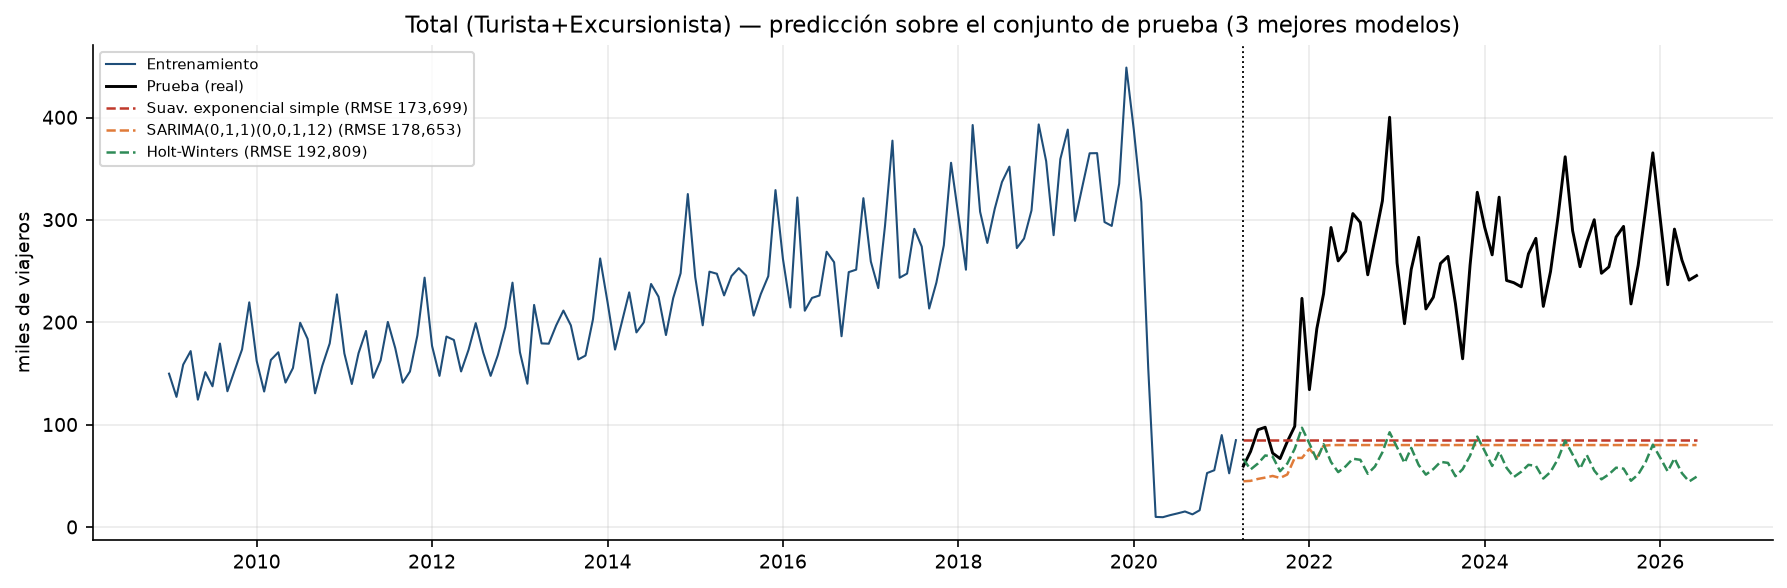
\includegraphics[width=\textwidth]{fig/24_total_pred.png}
\caption{Serie total: predicción de los tres mejores modelos sobre el conjunto de prueba. Todos
subestiman la recuperación porque el entrenamiento termina en el piso de la pandemia.}
\end{figure}

\subseccion{Control: partición alternativa post-pandemia}
\label{sec:control}

Para separar el error del choque exógeno del error propio del modelo, se repitió todo el
ejercicio entrenando desde \textbf{julio de 2021} (fronteras ya reabiertas) y dejando los
\textbf{últimos 18 meses} como prueba.

\begin{table}[H]
\centering
\small
\begin{tabular}{lcc|cc}
\toprule
& \multicolumn{2}{c|}{\textbf{Partición 70/30}} & \multicolumn{2}{c}{\textbf{Control post-pandemia}} \\
\textbf{Serie} & \textbf{Mejor modelo} & \textbf{MAPE \%} & \textbf{Mejor modelo} & \textbf{MAPE \%} \\
\midrule
Total (Tur.+Exc.)          & Suav. exp. simple & 60.6 & Seasonal naive            & \textbf{6.0} \\
Frontera: La Aurora        & Suav. exp. simple & 36.6 & SARIMA$(1,0,0)(1,0,0)_{12}$ & \textbf{8.3} \\
Frontera: Valle Nuevo      & Suav. exp. simple & 80.3 & Seasonal naive            & \textbf{12.7} \\
Frontera: San Cristóbal    & Suav. exp. simple & 81.5 & Seasonal naive            & \textbf{14.3} \\
Región: América Del Centro & Suav. exp. simple & 61.4 & Seasonal naive            & \textbf{9.8} \\
Región: América Del Norte  & Suav. exp. simple & 53.4 & Prophet                   & \textbf{7.2} \\
Región: Europa             & Suav. exp. simple & 71.4 & SARIMA$(1,0,1)(1,0,1)_{12}$ & \textbf{12.5} \\
\bottomrule
\end{tabular}
\caption{Comparación de las dos particiones. El error cae de 36--82\% a 6--14\% al eliminar el
quiebre estructural del conjunto de entrenamiento.}
\end{table}

\textbf{Este es el hallazgo metodológico central del laboratorio.} El MAPE cae de un rango de
\textbf{36--82\%} a un rango de \textbf{6--14\%}, una reducción de un orden de magnitud, sin
cambiar ni un solo modelo ni un solo dato. La conclusión es inequívoca: \textbf{el error de la
partición 70/30 no mide la calidad de los modelos, mide la magnitud del choque pandémico}.
Sobre datos homogéneos, estas series son \textbf{muy predecibles}: un error del 6--14\% a un
horizonte de 18 meses es un resultado sólido para planificación turística.

Nótese además que en el control cambian los ganadores y aparecen modelos con estructura
estacional ---seasonal naive, SARIMA con términos estacionales, Prophet---, exactamente lo
esperable en series con $F_S$ entre 0.42 y 0.88. El suavizamiento exponencial simple desaparece
del podio, confirmando que su victoria anterior era un accidente de la partición.

\subseccion{Análisis de residuos}

Se evaluaron los residuos del mejor SARIMA de cada serie con la prueba de \textbf{Ljung-Box}
($H_0$: los residuos son ruido blanco) y \textbf{Jarque-Bera} ($H_0$: son normales).

\begin{table}[H]
\centering
\small
\begin{tabular}{lccc}
\toprule
\textbf{Serie} & \textbf{Ljung-Box(12)} & \textbf{Ljung-Box(24)} & \textbf{¿Ruido blanco?} \\
\midrule
Total (Turista + Excursionista) & 0.274 & --- & Sí \\
Frontera: La Aurora             & 0.025 & --- & Marginal \\
Frontera: Valle Nuevo           & 0.048 & --- & Marginal \\
Frontera: San Cristóbal         & 0.045 & --- & Marginal \\
Región: América Del Centro      & 0.285 & --- & Sí \\
Región: América Del Norte       & 0.000 & 0.000 & \textbf{No} \\
Región: Europa                  & 0.000 & 0.000 & \textbf{No} \\
\bottomrule
\end{tabular}
\caption{Valores $p$ de Ljung-Box sobre los residuos del mejor SARIMA de cada serie.}
\end{table}

\textbf{Interpretación honesta de estos resultados.} En las dos series agregadas los residuos
son ruido blanco: el modelo ha extraído toda la estructura disponible. En las tres fronteras el
resultado es marginal (valores $p$ entre 0.025 y 0.048), lo que indica algo de autocorrelación
residual, atribuible en buena medida a la \textbf{Semana Santa}: al ser una fiesta móvil que
salta entre marzo y abril, un modelo estacional de período fijo 12 no puede capturarla y deja
residuo sistemático en esos meses.

En \textbf{América del Norte y Europa el modelo es claramente inadecuado} ($p = 0.000$). La
causa es identificable: son las dos únicas series con \textbf{cinco meses en cero} (abril a
agosto de 2020, cuando el ingreso de extranjeros fue literalmente nulo). En escala logarítmica
ese cero es un salto de magnitud enorme respecto del nivel habitual, y ningún SARIMA lineal
puede absorberlo. \textbf{El tratamiento correcto sería incorporar variables dummy de
intervención} para la ventana de cierre (un modelo ARIMAX), o tratar esos meses como
\textit{no observados} en lugar de como ceros, dado que la frontera cerrada significa que la
demanda no se midió, no que fuera cero. Se deja explícitamente señalado como la principal
limitación del modelado de estas dos series.

En las siete series la prueba de \textbf{Jarque-Bera rechaza la normalidad} ($p < 0.001$), lo
que era esperable: los residuos de 2020 son valores extremos genuinos. Esto no invalida las
predicciones puntuales, pero sí implica que \textbf{los intervalos de confianza calculados bajo
el supuesto de normalidad son demasiado estrechos} y no deben tomarse al pie de la letra.

\begin{figure}[H]
\centering
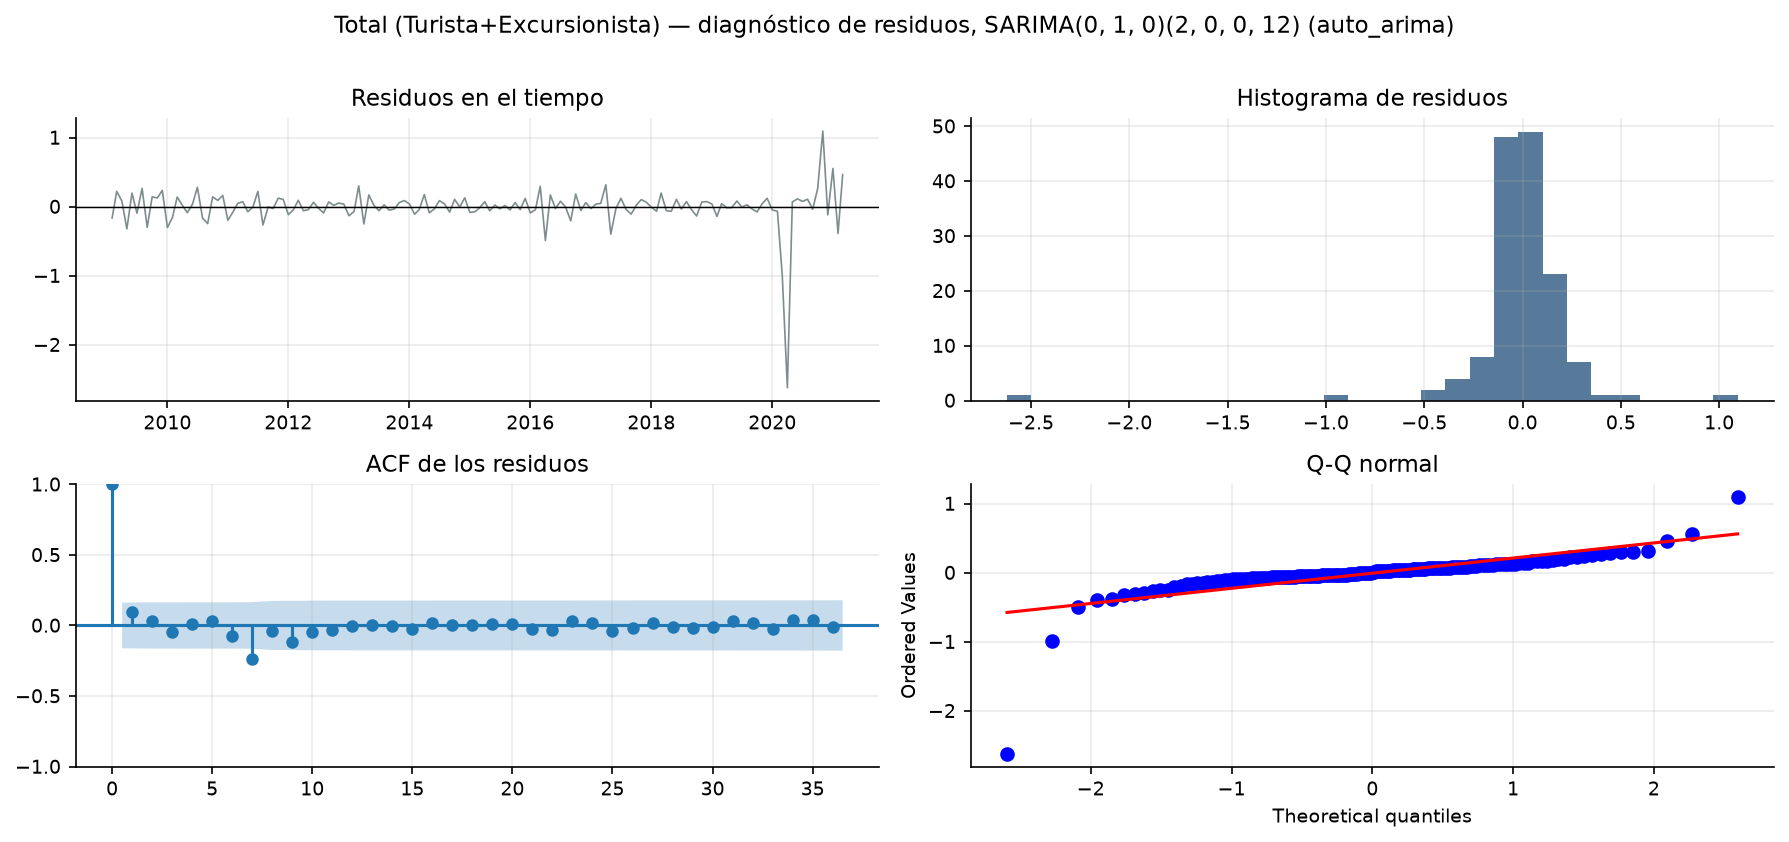
\includegraphics[width=\textwidth]{fig/25_total_residuos.png}
\caption{Serie total: diagnóstico de residuos del mejor SARIMA. La ACF de los residuos no
muestra estructura remanente; el Q-Q evidencia las colas pesadas de la pandemia.}
\end{figure}

\subseccion{Comparación detallada por serie}

A continuación se presenta la tabla completa de modelos para la serie obligatoria. Las tablas de
las seis series restantes siguen el mismo formato y están en el cuaderno de análisis.

\begin{table}[H]
\centering
\small
\begin{tabular}{lrrrrrr}
\toprule
\textbf{Modelo} & \textbf{AIC} & \textbf{BIC} & $\boldsymbol{n_{\text{ef}}}$ & \textbf{MAE} & \textbf{RMSE} & \textbf{MAPE} \\
\midrule
Suav. exponencial simple             & $-326.1$ & $-320.1$ & 147 & 158{,}767 & 173{,}699 & 60.6 \\
SARIMA$(0,1,1)(0,0,1)_{12}$          & 86.9 & 95.6 & 146 & 163{,}231 & 176{,}622 & 63.5 \\
Holt-Winters                         & $-354.3$ & $-306.4$ & 147 & 178{,}380 & 192{,}809 & 68.6 \\
SARIMA$(2,1,0)(1,0,0)_{12}$          & 79.8 & 91.4 & 146 & 197{,}207 & 209{,}470 & 79.6 \\
Seasonal naive                       & --- & --- & 147 & 207{,}293 & 219{,}634 & 84.9 \\
SARIMA$(1,1,1)(1,0,1)_{12}$          & 70.9 & 85.3 & 146 & 208{,}232 & 223{,}054 & 82.0 \\
SARIMA$(1,1,1)(0,1,1)_{12}$          & 70.6 & 81.7 & 134 & 213{,}023 & 227{,}948 & 84.1 \\
SARIMA$(0,1,1)(0,1,1)_{12}$          & 68.9 & 77.2 & 134 & 213{,}851 & 228{,}724 & 84.5 \\
SARIMA$(0,1,0)(2,0,0)_{12}$ \small{(auto)} & \textbf{58.8} & \textbf{67.2} & 146 & 217{,}446 & 237{,}176 & 83.0 \\
Prophet                              & --- & --- & 147 & 240{,}279 & 252{,}691 & 98.2 \\
\bottomrule
\end{tabular}
\caption{Serie total: comparación de los diez modelos, ordenados por RMSE sobre el conjunto de
prueba. Recuérdese que AIC y BIC solo son comparables dentro del mismo $n_{\text{ef}}$.}
\end{table}

\textbf{Lectura de la tabla, y por qué AIC y RMSE apuntan en direcciones opuestas.} Dentro del
grupo $n_{\text{ef}} = 146$, el mejor modelo por \textbf{AIC y BIC} es
SARIMA$(0,1,0)(2,0,0)_{12}$, el que propone \texttt{auto\_arima}, y sus residuos son ruido
blanco ($p = 0.274$). Sin embargo, ese mismo modelo queda \textbf{penúltimo por RMSE}. No hay
contradicción: \textbf{el AIC mide el ajuste dentro de la muestra de entrenamiento y el RMSE
mide el error fuera de ella}. El modelo describe muy bien el período 2009--2021 ---incluida la
pandemia--- y precisamente por eso proyecta hacia adelante un nivel deprimido. El criterio
correcto para \textbf{seleccionar un modelo de pronóstico es el error fuera de muestra}, pero en
este caso ese error está dominado por el quiebre estructural, y por eso la decisión final se
apoya en la partición de control de la sección~\ref{sec:control}.

%======================= 6. ANALISIS COMPARATIVO =======================
\seccion{Análisis comparativo (punto 5)}

\subseccion{Criterios de medición}

Cada pregunta se responde con un estadístico explícito, para que la comparación sea reproducible
y no dependa de la lectura visual de los gráficos.

\begin{table}[H]
\centering
\small
\begin{tabularx}{\textwidth}{lX}
\toprule
\textbf{Pregunta} & \textbf{Estadístico} \\
\midrule
Mayor estacionalidad & Fuerza estacional $F_S$ de la descomposición STL (2009--2019) \\
Mayor tendencia de crecimiento & Tasa de crecimiento anual compuesta (TCAC) 2009--2019 \\
Mayor volatilidad & Desviación estándar de $\log(y_t / y_{t-12})$ (2009--2019) \\
Más afectada por la pandemia & Caída del total de 2020 respecto de 2019 y nivel de 2025 vs. 2019 \\
\bottomrule
\end{tabularx}
\end{table}

\begin{table}[H]
\centering
\small
\begin{tabular}{lcccc|cc}
\toprule
& & & & & \multicolumn{2}{c}{\textbf{2025 vs 2019 \%}} \\
\textbf{Serie} & $\boldsymbol{F_S}$ & \textbf{TCAC \%} & \textbf{Volat.} & \textbf{Caída 2020 \%} & \textbf{cruda} & \textbf{homog.} \\
\midrule
Total (Turista + Excursionista) & 0.795 & 8.19 & 0.105 & $-74.4$ & 81.2 & 138.2 \\
\midrule
Frontera: La Aurora      & \textbf{0.874} & 4.74 & 0.074 & $-72.8$ & 80.3 & 147.8 \\
Frontera: Valle Nuevo    & 0.421 & 9.69 & \textbf{0.373} & $\mathbf{-80.7}$ & 71.7 & \textbf{106.6} \\
Frontera: San Cristóbal  & 0.706 & \textbf{12.95} & 0.304 & $-72.6$ & 90.2 & 159.1 \\
\midrule
Región: América Del Centro & 0.805 & \textbf{9.83} & \textbf{0.122} & $\mathbf{-74.4}$ & 66.0 & 138.8 \\
Región: América Del Norte  & \textbf{0.882} & 3.82 & 0.106 & $-74.1$ & 139.3 & 139.3 \\
Región: Europa             & 0.880 & 2.23 & 0.110 & $-71.9$ & 125.8 & \textbf{125.8} \\
\bottomrule
\end{tabular}
\caption{Comparación entre series. En negrita el máximo (o mínimo, según corresponda) dentro de
cada categoría. La columna \textbf{cruda} compara un 2019 que incluye residentes de Guatemala
contra un 2025 que no; la \textbf{homogénea} los excluye de ambos años y es la única
interpretable. En América del Norte y Europa ambas coinciden porque esas regiones nunca
contuvieron residentes guatemaltecos.}
\end{table}

\begin{figure}[H]
\centering
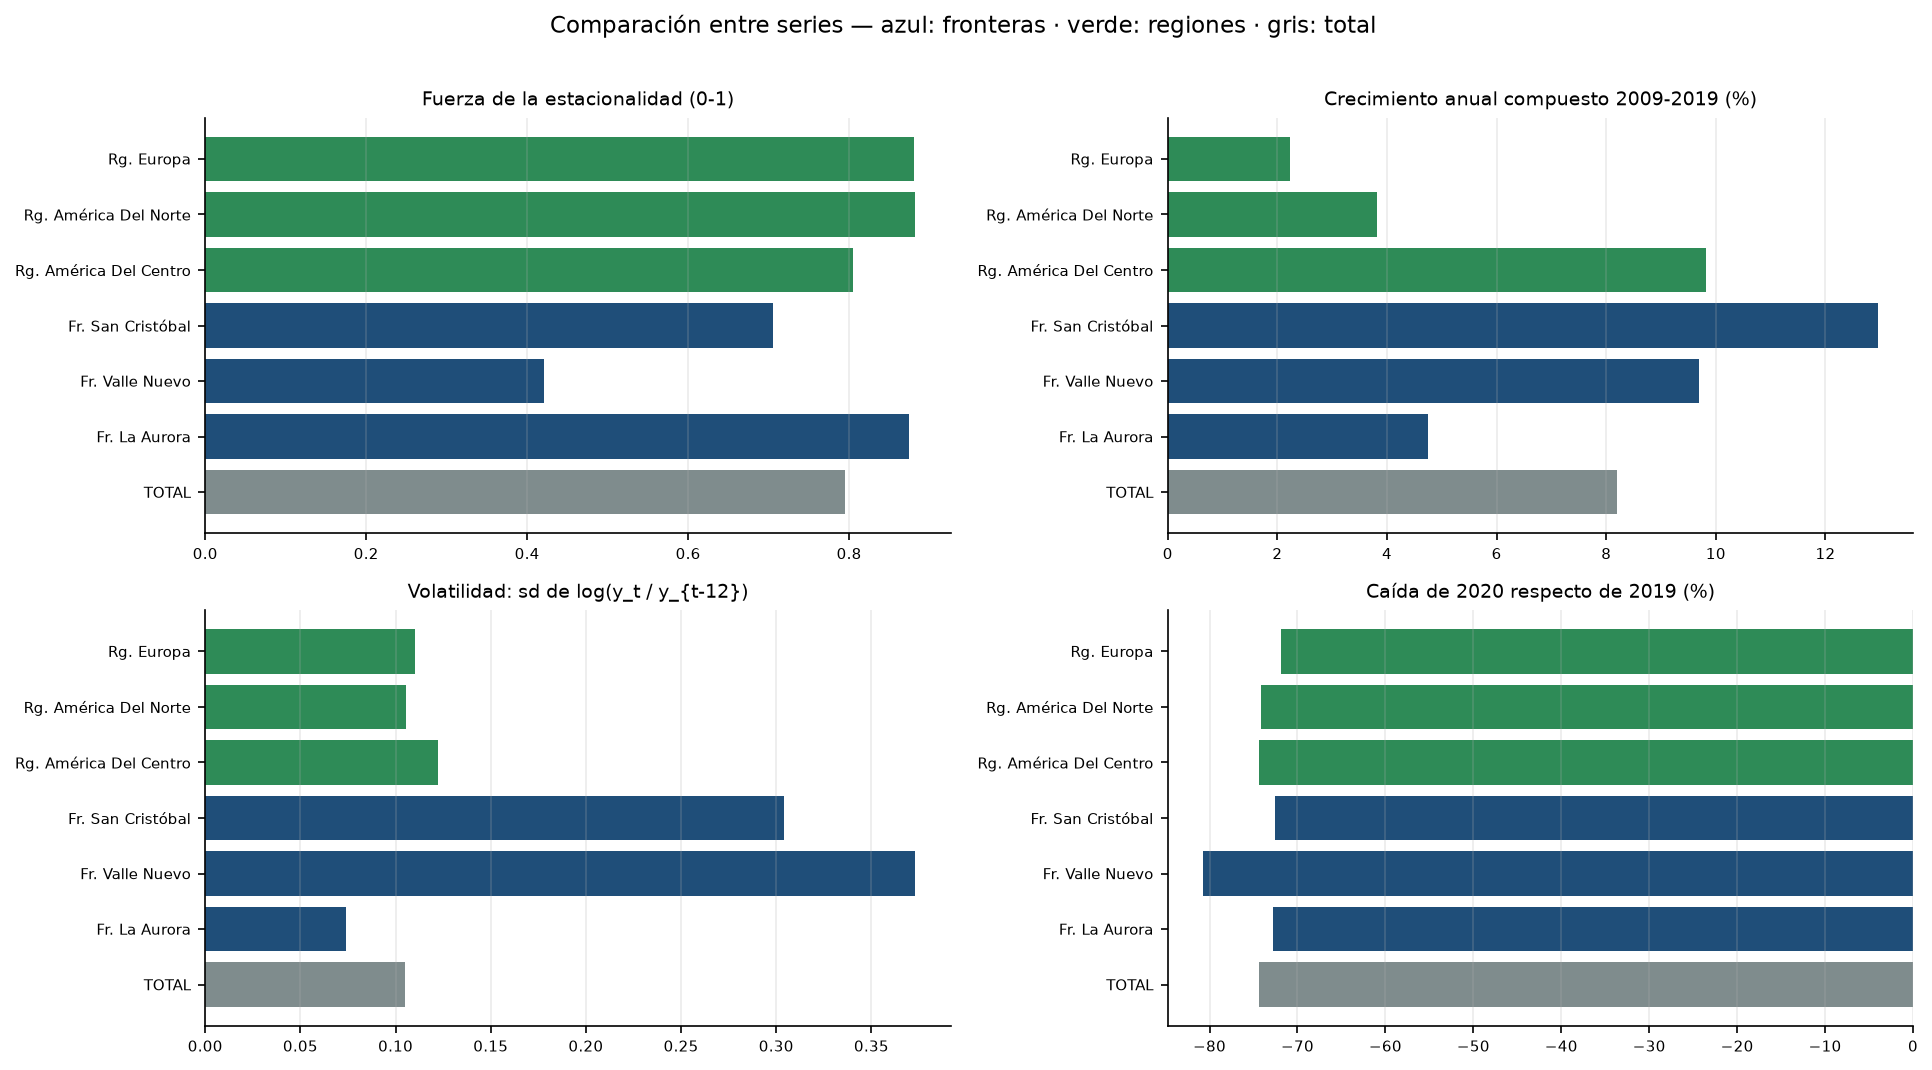
\includegraphics[width=\textwidth]{fig/30_comparativo.png}
\caption{Comparación visual de los cuatro criterios. Azul: fronteras; verde: regiones;
gris: total.}
\end{figure}

\subseccion{Respuestas por categoría}

\textbf{Categoría 1 --- Fronteras}

\begin{enumerate}[label=\roman*.,leftmargin=1.8em,itemsep=4pt]
  \item \textbf{Mayor estacionalidad: La Aurora} ($F_S = 0.874$). El aeropuerto tiene el patrón
  anual más marcado y regular, coherente con un flujo dominado por vacaciones planificadas y
  visita de la diáspora en diciembre. Valle Nuevo, en cambio, es la menos estacional
  ($F_S = 0.421$): el tránsito terrestre con El Salvador tiene un componente cotidiano y
  comercial que no depende de la temporada.
  \item \textbf{Mayor tendencia de crecimiento: San Cristóbal} (TCAC $= 12.95\%$ anual
  2009--2019). Casi triplica el ritmo de La Aurora (4.74\%). Es el corredor con Honduras y el de
  mayor dinamismo estructural del período.
  \item \textbf{Mayor volatilidad: Valle Nuevo} (sd de la tasa interanual $= 0.373$), cinco
  veces la de La Aurora (0.074). El flujo aéreo es el más estable y predecible; el terrestre con
  El Salvador, el más errático.
  \item \textbf{Más afectada por la pandemia: Valle Nuevo}, con una caída del \textbf{80.7\%} en
  2020 frente a 2019 ---la única que superó el 80\%--- y además la \textbf{peor recuperada}: a
  definición homogénea está en el \textbf{106.6\%} de 2019, apenas por encima del nivel
  prepandemia, mientras La Aurora alcanza el 147.8\% y San Cristóbal el 159.1\%. El orden de las
  tres fronteras es el mismo con la comparación cruda (71.7\%, 80.3\% y 90.2\%), de modo que
  \textbf{esta respuesta no depende del criterio}: cambia la magnitud, no el diagnóstico. Las
  tres tocaron un piso cercano al $-100\%$ en el peor mes; lo que las distingue es la velocidad
  de recuperación.
\end{enumerate}

\textbf{Categoría 2 --- Regiones geográficas}

\begin{enumerate}[label=\roman*.,leftmargin=1.8em,itemsep=4pt]
  \item \textbf{Mayor estacionalidad: América del Norte} ($F_S = 0.882$), seguida muy de cerca
  por Europa (0.880). Ambos son mercados de larga distancia con temporadas bien definidas
  (verano boreal e invierno). América Central es la menos estacional (0.805), por su componente
  de viaje regional frecuente.
  \item \textbf{Mayor tendencia de crecimiento: América Central} (TCAC $= 9.83\%$), muy por
  encima de América del Norte (3.82\%) y Europa (2.23\%). Confirma el hallazgo del exploratorio:
  \textbf{el crecimiento del turismo guatemalteco fue regional, no de larga distancia}.
  \item \textbf{Mayor volatilidad: América Central} (0.122), aunque las tres regiones son
  notablemente parecidas (0.106--0.122). A nivel regional los flujos se promedian entre muchos
  puntos de entrada y la volatilidad se diluye; es a nivel de frontera individual donde aparecen
  las diferencias grandes.
  \item \textbf{Más afectada en 2020: América Central}, con una caída del \textbf{74.4\%},
  seguida muy de cerca por América del Norte ($-74.1\%$) y Europa ($-71.9\%$). Las tres son
  prácticamente indistinguibles: el cierre de fronteras fue indiscriminado. \textbf{Peor
  recuperada: Europa}, con un \textbf{125.8\%} del nivel de 2019, frente a 138.8\% de América
  Central y 139.3\% de América del Norte. Las tres superan su nivel prepandemia.
\end{enumerate}

\textbf{Advertencia imprescindible: en esta categoría la respuesta cambia según el criterio.}
Con la comparación \textbf{cruda}, América Central aparece como la peor recuperada con un
66.0\%, y era la respuesta que arrojaba un primer análisis. \textbf{Es falsa.} América Central
es precisamente la región donde estaban clasificados los residentes de Guatemala, que
representaban el \textbf{52.5\% de la región en 2019} y desaparecen del conteo desde 2023. Al
comparar un 2019 que los incluye contra un 2025 que no, se mide el cambio de definición y no la
demanda:

\begin{table}[H]
\centering
\small
\begin{tabular}{lrrr}
\toprule
\textbf{América Central} & \textbf{Total} & \textbf{Residentes de Guatemala} & \textbf{Sin Guatemala} \\
\midrule
2019 & 3{,}247{,}484 & 1{,}703{,}434 (52.5\%) & 1{,}544{,}050 \\
2025 & 2{,}143{,}511 & 0 (0\%) & 2{,}143{,}511 \\
\midrule
2025 / 2019 & \textit{66.0\% (engañoso)} & --- & \textbf{138.8\%} \\
\bottomrule
\end{tabular}
\caption{El ``desplome'' de América Central es enteramente un artefacto de definición: a
definición constante la región creció un 38.8\% sobre 2019.}
\end{table}

En cambio, las cifras de \textbf{América del Norte y Europa no requieren corrección}: ninguna
de las dos contuvo nunca residentes guatemaltecos, y su composición interna se mantiene
comparable ---América del Norte conserva las mismas tres categorías (Estados Unidos, México,
Canadá) en 2019 y en 2025, y en Europa la agregación de mercados de 2023 reagrupó países
\textit{dentro} de la misma región, sin trasvasar volumen a otras. Sus crecimientos del 39\% y
26\% sobre 2019 son \textbf{reales}.

La lección general es que \textbf{ninguna comparación con años anteriores a 2023 es válida sin
homogeneizar antes la definición}, y que hacerlo puede invertir por completo la conclusión.

%======================= 7. CONCLUSIONES =======================
\seccion{Hallazgos útiles para el INGUAT (punto 5.b)}

\begin{enumerate}[leftmargin=1.6em,itemsep=6pt]

\item \textbf{Las estadísticas oficiales tienen dos rupturas de serie que invalidan cualquier
comparación directa 2022 vs. 2023.} El total agregado aparenta caer 25\%, pero se debe a un
cambio de definición y a la salida de los residentes guatemaltecos del conteo, no a una pérdida
de demanda turística. \textbf{Recomendación operativa:} publicar la serie
\textit{Turista + Excursionista} como indicador oficial de continuidad y documentar el quiebre.
Si no se hace, cualquier informe de gestión que compare esos años estará reportando una caída
que no ocurrió.

\item \textbf{El turismo extranjero sí se recuperó, y con holgura: la ``caída del 19\%'' no
existe.} Es el hallazgo más importante del informe porque contradice la lectura directa de los
datos. La cifra de que 2025 está en el 81\% del nivel de 2019 compara un 2019 que incluye a
1.7 millones de residentes guatemaltecos retornantes contra un 2025 que ya no los cuenta. A
definición homogénea, \textbf{2025 está en el 138\% de 2019} (+38\%, un 5.5\% anual compuesto).
\textbf{Recomendación:} el INGUAT no debe reportar caídas ni diseñar planes de reactivación
sobre esa comparación. Lo que cayó es la cobertura del indicador, no la demanda. El único dato
de desaceleración genuino ---y homogéneo, porque compara dos años posteriores al quiebre--- es
que el primer semestre de 2026 va \textbf{3\% por debajo} del mismo semestre de 2025; eso sí
merece seguimiento.

\item \textbf{Tres puestos fronterizos concentran el 71\% del flujo.} La Aurora (40.7\%), Valle
Nuevo (21.7\%) y San Cristóbal (9.0\%). Un plan de capacidad, señalización, migración o
promoción concentrado en esos tres puntos cubre casi tres cuartas partes del movimiento del
país con una fracción del presupuesto de una intervención nacional.

\item \textbf{El crecimiento es regional y terrestre, no de larga distancia.} América Central
creció al 9.83\% anual entre 2009 y 2019, frente al 3.82\% de América del Norte y el 2.23\% de
Europa. \textbf{Implicación de política:} el presupuesto de promoción internacional debería
reflejar esta asimetría. El mercado que sostiene el volumen es el vecino, y es además el más
barato de captar.

\item \textbf{Valle Nuevo es el punto que exige atención prioritaria.} Es simultáneamente la
frontera \textbf{más afectada} por la pandemia ($-80.7\%$ en 2020), la \textbf{peor recuperada}
(106.6\% del nivel de 2019 a definición homogénea, cuando las otras dos superan el 147\%) y la
\textbf{más volátil} (cinco veces La Aurora). Concentra el problema y la incertidumbre a la vez,
y su diagnóstico es robusto: sale peor con cualquiera de los dos criterios de comparación.

\item \textbf{San Cristóbal es la oportunidad de crecimiento.} Mayor tendencia de todas
(12.95\% anual 2009--2019) y mejor recuperación (159.1\% de 2019 a definición homogénea). Es el
corredor con Honduras y el de mayor dinamismo estructural del país; conviene acompañar ese
crecimiento con inversión en capacidad antes de que se sature.

\item \textbf{La estacionalidad sobrevivió intacta a la pandemia; el nivel no.} El patrón anual
---máximo en diciembre (índice 134), mínimos en febrero (81) y septiembre (83), amplitud de 53
puntos--- se mantiene idéntico después de 2021, solo que a menor escala. \textbf{Esto es una
buena noticia operativa:} significa que la planificación de personal, turnos migratorios y
capacidad hotelera por temporada sigue siendo válida con el calendario histórico; lo único que
cambió es el volumen base.

\item \textbf{Estas series son altamente predecibles sobre datos homogéneos.} La partición de
control demuestra un \textbf{MAPE de 6--14\% a 18 meses vista}, un margen perfectamente
utilizable para presupuestar y dimensionar operaciones. El error del 36--82\% de la partición
oficial mide el choque pandémico, no la calidad de los modelos.

\item \textbf{Los modelos más simples con estructura estacional son suficientes.} En el control
post-pandemia, el \textbf{seasonal naive} ---predecir el mismo mes del año anterior--- gana en
cuatro de las siete series. \textbf{Implicación práctica:} el INGUAT no necesita infraestructura
analítica sofisticada para obtener pronósticos útiles; necesita series limpias y sin rupturas de
definición. El cuello de botella es la calidad del dato, no el algoritmo.

\item \textbf{Recomendación de medición.} Los meses de frontera cerrada deberían registrarse
como \textit{no medidos}, no como cero. Tal como están, distorsionan el modelado de América del
Norte y Europa hasta el punto de que ningún SARIMA lineal logra residuos de ruido blanco. Es una
corrección de bajo costo y alto impacto para el uso analítico futuro de la base.

\end{enumerate}

\subseccion{Limitaciones del estudio}

\begin{itemize}[leftmargin=1.4em,itemsep=3pt]
  \item La partición 70/30 que exige el enunciado corta \textbf{dentro del hueco pandémico}, lo
  que hace que las métricas de error de la sección 5.1 no sean informativas sobre la calidad de
  los modelos. Se mitigó con la partición de control, pero es una limitación de diseño.
  \item Los modelos de \textbf{América del Norte y Europa} dejan autocorrelación residual
  significativa por los cinco meses en cero de 2020. Requerirían un ARIMAX con variables de
  intervención, fuera del alcance de este laboratorio.
  \item La \textbf{Semana Santa} es una fiesta móvil entre marzo y abril y ningún modelo
  estacional de período fijo 12 la captura; explica parte del residuo de las series de frontera.
  \item Toda comparación que cruce el año \textbf{2023} exige homogeneizar la definición antes
  de interpretarla. En este informe se hizo excluyendo a los residentes de Guatemala de ambos
  extremos; es la corrección de primer orden y explica la práctica totalidad de la discrepancia,
  pero no captura efectos residuales de la reagrupación de mercados dentro de cada región.
  \item Los datos son \textbf{de uso académico} y no corresponden a cifras oficiales del INGUAT
  ni del Instituto Guatemalteco de Migración.
\end{itemize}

\vspace{1em}
\hrule
\vspace{0.6em}
{\small \textbf{Repositorio del código:}
\url{https://github.com/rodrigoajmac/CC3084_Laboratorio_1}

\vspace{0.4em}
Los cuadernos \texttt{01\_EDA\_series\_tiempo.ipynb},
\texttt{02\_Analysis\_TimeSeries.ipynb} y \texttt{03\_Modelado\_Prediccion.ipynb} contienen el
análisis exploratorio, la exploración inicial de series alternativas y el modelado completo,
respectivamente.}

\end{document}
